\documentclass[12pt,final,fleqn]{article}

% basic packages
\usepackage[margin=1in] { geometry }
\usepackage{amssymb,amsmath, bm}
\usepackage{verbatim}
\usepackage[utf8]{inputenc}
%\usepackage[OT1]{fontenc}
\usepackage{setspace}
\usepackage{enumitem}
\usepackage[bottom]{footmisc}
\usepackage{url}
\usepackage[font={bf}]{caption}
\usepackage{float}
%\usepackage{pgfplots}
%\usepackage[font={bf}]{caption}
\usepackage{setspace}
\usepackage{latexsym}
%\usepackage{euscript}
\usepackage{graphicx}
\usepackage{marvosym}
\usepackage{amsmath} 
\usepackage{authblk}
\usepackage{xcolor}
\usepackage{blindtext}
%\usepackage[varg]{txfonts}  Older version of ``g'' in math. 
\usepackage{changepage}

\usepackage{epigraph}

% bibliography packages
\usepackage[natbibapa]{apacite}
\bibliographystyle{apsr}
\bibpunct{(}{)}{;}{a}{}{,}
\renewcommand{\bibname}{References}

% packages for tables
\usepackage{booktabs}
\usepackage{longtable}
\usepackage{caption}
\usepackage{array}
\usepackage{multirow}
\usepackage{wrapfig}
\usepackage{float}
\usepackage{colortbl}
\usepackage{pdflscape}
\usepackage{tabu}
\usepackage{threeparttable}
\usepackage{threeparttablex}
\usepackage[normalem]{ulem}
\usepackage{makecell}
\usepackage{xcolor}
\usepackage{siunitx}
\newcolumntype{d}{S[input-symbols = ()]}

\usepackage{booktabs, threeparttable}
%\usepackage{tabularx}
% dcolumn package
\usepackage{dcolumn}
\newcolumntype{.}{D{.}{.}{-1}}
\newcolumntype{d}[1]{D{.}{.}{#1}}
\captionsetup{belowskip=10pt,aboveskip=5pt}
\usepackage{multirow}
% rotating package
\usepackage[figuresright]{rotating}
\usepackage{pdflscape}
\usepackage{subcaption}

% packages for figures
\usepackage{grffile}
\usepackage{afterpage}
\usepackage{float}
\usepackage[section]{placeins}
\usepackage{caption}

% theorem package
\usepackage{theorem}
\theoremstyle{plain}
\theoremheaderfont{\scshape}
\newtheorem{theorem}{Theorem}
\newtheorem{algorithm}{Algorithm}
\newtheorem{assumption}{Assumption}
\newtheorem{lemma}{Lemma}
\newtheorem{proposition}{Proposition}
\newtheorem{remark}{Remark}
\newcommand{\qed}{\hfill \ensuremath{\Box}}
\newcommand\indep{\protect\mathpalette{\protect\independenT}{\perp}}
\DeclareMathOperator{\sgn}{sgn}
\DeclareMathOperator{\tr}{tr}
\DeclareMathOperator{\argmin}{arg\min}
\DeclareMathOperator{\argmax}{arg\max}
\def\independenT#1#2{\mathrel{\rlap{$#1#2$}\mkern2mu{#1#2}}}
\providecommand{\norm}[1]{\lVert#1\rVert}
\renewcommand\r{\right}
\renewcommand\l{\left}
\newcommand\E{\mathbb{E}}
\newcommand\dist{\buildrel\rm d\over\sim}
\newcommand\iid{\stackrel{\rm i.i.d.}{\sim}}
\newcommand\ind{\stackrel{\rm indep.}{\sim}}
\newcommand\cov{{\rm Cov}}
\newcommand\var{{\rm Var}}
\newcommand\SD{{\rm SD}}
\newcommand\bone{\mathbf{1}}
\newcommand\bzero{\mathbf{0}}

% dotted lines in tables
%\usepackage{arydshln}

\usepackage{pdflscape}
\usepackage{pdfpages}

% spacing between sections and subsections
\usepackage[compact]{titlesec}

% hyperref options
\usepackage{color}
\usepackage{hyperref}
\usepackage{xcolor}
\hypersetup{
    colorlinks,
    linkcolor={blue!50!black},
    citecolor={blue!50!black},
    urlcolor={blue!80!black}
}
%\newcommand*{\Appendixautorefname}{Appendix}
%\renewcommand*{\sectionautorefname}{Section}
%\renewcommand*{\subsectionautorefname}{Section}
%\newcommand{\aref}[1]{\hyperref[#1]{Appendix~\ref{#1}}}

% times new roman
%\usepackage{times}

% appendix settings
\usepackage[toc,page,header]{appendix}
\usepackage{minitoc}
\mtcsetfeature{minitoc}{open}{\vspace*{1cm}}
\renewcommand\ptctitle{ }
\renewcommand{\appendixpagename}{\centering Appendices}
\usepackage{chngcntr}
\usepackage{etoolbox}
\usepackage{lipsum}

\setcounter{secnumdepth}{0}

% file paths and definitions
\makeatletter
\newcommand*\ExpandableInput[1]{\@@input#1 }
\makeatother

\setlength{\mathindent}{1cm}
\allowdisplaybreaks[4]
\doublespacing
%\special{pdf: pagesize width 8.5truein height 11.0truein}

\titleformat{\subsection}
  {\itshape\large}{\thesubsection}{1em}{}

% Table of contents settings
%\setcounter{tocdepth}{1}

% Make the "Part I" text invisible
\renewcommand \thepart{}
\renewcommand \partname{}


%--------------------------------------------------------------------------------------
% BEGIN DOCUMENT
%--------------------------------------------------------------------------------------

\begin{document}
\singlespace
\title{\textbf{Countering capture in local politics: \\ Evidence from eight field experiments}\thanks{I extend a special thank you to Abundant Housing LA, my partner in the implementation of this project. I also thank CSAP and ISPS at Yale University for generous support; P.M. Aronow, Moritz Bondeli, David Broockman, Alex Coppock, Charles Crabtree, Katherine Einstein, Matthew Graham, Gregory Huber, Devin Incerti, Joshua Kalla, Colin Moreshead, Mina Pollmann, Frances Rosenbluth, Kenneth Scheve, Hikaru Yamagishi, and three anonymous reviewers for invaluable feedback; and participants at the Yale Leitner Seminar in Political Economy, Junior Americanist Workshop Series, and the Toronto Political Behavior Workshop. The human subject protocol of the research was evaluated and approved by an ethics committee at Yale University (IRB Protocol ID \#2000030461). The research design and analyses were pre-registered at: \url{https://osf.io/c84j7}. Any and all errors are my own.}}

\author{Trevor Incerti\thanks{Assistant Professor, Department of Political Science, University of Amsterdam}}
\date{\today}

\doparttoc % Tell to minitoc to generate a toc for the parts
\faketableofcontents % Run a fake tableofcontents command for the partocs
 
\part{} % Start the document part
\parttoc % Insert the document TOC

\maketitle
\thispagestyle{empty}

\begin{abstract}
\noindent
In the first field experiments to encourage participation in local civic bodies, I examine if outreach can reduce inequalities in who participates in city council meetings. Renter participation in local politics lags that of homeowners, who often participate to oppose housing growth. 19,951 renter households received randomly assigned emails encouraging them to comment at their city council meetings and support housing growth. Opening a message highlighting potential costs of abstention from local politics increased public comments by 1.4 percentage points versus placebo. These effects are substantively large: treatment-induced comments represented 8\% of total comments and 46\% of pro-housing comments across all targeted meetings. The results suggest that even low-cost outreach strategies can meaningfully increase participation in lesser-known settings like city councils and make these bodies more reflective of the general public. Further, increasing the perception that abstention is costly appears to be an effective motivator of collective action.

\end{abstract} 

%\vspace{0.5cm}
%\begin{center}
%Word count: 4400 words
%\end{center}


\setcounter{page}{0}
\pagebreak
\doublespace
%\singlespace

Homeowner participation in local politics in the United States outpaces that of renters \citep{yoder2020does, hall2018does, einstein2019participates}. Even moving city council meetings online in 2020 did not increase renter attendance \citep{einstein2021zoom}. Research into local housing policy suggests that this participation gap is reflected in land use and zoning policies that represent the economic interests of homeowners \citep{fischel2005homevoter, einstein2019neighborhood, marble2021self}. Yet these policies often harm renters through decreased access to housing and higher rents \citep{glaeser2005have, glaeser2018economic, charette2015projecting, ganong2017has, lens2016strict, glaeser2002impact, quigley2005effects}. Renters therefore also have an incentive to participate in local politics and support housing growth, but their participation lags homeowners. 

Differences in economic incentives partially explain this participatory gap. Economic self-interest typically only motivates political behavior when benefits are ``tangible, large, visible, and certain'' \citep{citrin1990american}. Homeowners can receive tangible benefits from halting neighboring development through preserved property value. For renters, more housing will only reduce rents throughout a diffuse geographic region in the long term. How then can those who only benefit through long-term and uncertain gains (like renters) be motivated to engage in personally costly political behavior?

In the first field experiments to motivate participation in local civic bodies, 19,951 renter households in 8 cities in Los Angeles (LA) County were randomly assigned to receive emails encouraging them to comment at their city council meetings and support pro-housing regulatory policies.  Three mechanisms of mobilization were tested by randomizing messaging to: (1) provide attendance instructions only, (2) prime rational economic self interest, or (3) highlight the costs of abstention from local politics. 

Receipt of any treatment increased public comments by 1 percentage point (pp) versus placebo, while highlighting costs of abstention increased comments by 1.4pp. Voters in local elections were more responsive to treatment (2.3pp) than non-voters (0.9pp). These effects are substantively large as council meeting attendance is typically low. Treatment-induced comments comprised 8\% of total comments and 46\% of pro-housing comments across all meetings. A majority of comments were pro-housing in over 50\% of treated meetings, in stark contrast with previous findings that pro-housing comments are typically in the minority in council meetings in equilibrium \citep{einstein2021zoom, yoder2020does}.

These results suggest that in direct contrast with voter turnout, low-cost outreach strategies like email can meaningfully increase political participation in remote settings such as commenting at city council meetings. As council meetings have low baseline rates of attendance, the increases in participation caused by this outreach are substantively large. Outreach targeted at underrepresented groups can therefore make civic bodies more reflective of the broader public, unlike allowing remote access alone. In terms of messaging, increasing perceived costs of abstention appears to be a particularly effective motivator of participation. 


\section{Homeownership and political participation}

This paper examines if direct outreach can make participation in local civic bodies more reflective of the broader public.\footnote{Similar outreach campaigns could also be used on different populations to increase participatory gaps. However, due to pre-existing asymmetries in information and incentives, it is unclear if such campaigns would be as effective as those contacting underrepresented groups. Further research is necessary to establish how high-participation groups are mobilized.} Research using administrative data finds that becoming a homeowner increases individuals' propensity to vote in local elections or participate in city council, planning, and zoning meetings \citep{yoder2020does, hall2018does}. Examination of the mechanisms driving  homeowner participation suggests this behavior is consistent with rational economic behavior in the form of protection of property values \citep{yoder2020does, hall2018does, mccabe2016no, marble2021self}. Homeowners are more likely to support policies that restrict new housing development, raising the value of existing homes \citep{hankinson2018renters, einstein2019participates}.\footnote{From an economic policy perspective, the ability of residents to block new housing construction is regularly cited as a key cause of decreases in housing supply \citep{glaeser2005have}. These supply restrictions are estimated to reduce geographic mobility, reduce real income for renters, and lower aggregate US economic growth \citep{glaeser2018economic, hsieh2019housing}.} 

The makeup of local political participation in majority-renter cities therefore does not typically reflect general public opinion. Unlike homeowners, renters do not consistently oppose new housing \citep{marble2021self, hankinson2018renters, monkkonen2019opposition}.  This leads to discrepancies between the percentage of council meeting comments in favor of additional housing and the percentage of ballots cast in favor of additional housing \citep{einstein2019participates}. Even moving council meetings online due to COVID-19 did not reduce the participation gap between renters and homeowners  \citep{einstein2021zoom}. However, while increased access did not increase renter participation, it remains unclear if making the economics of housing policy salient for renters would increase their participation, just as homeownership causes participation to increase through economic channels.\footnote{Participation is also highly unequal in project-by-project approval institutions such as city planning and zoning meetings. While project approval often occurs within city councils in the LA area, this is not always the case. Whether outreach campaigns are also effective at increasing turnout in more bureaucratic settings such as planning and zoning meetings is an important area for future research.} 


\section{Encouraging remote political participation}\label{theory: renters}


City council participation was limited to email, phone, or video calls due to COVID-19 at the time of the experiment, and these remote options remain in place to this day. Remote access did not, however, reduce pre-existing participatory gaps \citep{einstein2021zoom}, and prior research offers both lessons and conflicting predictions for encouraging remote political participation. 

Experimental research primarily finds digital outreach ineffective for in-person political mobilization \citep{green2019get}. However, tests of the efficacy of digital outreach at increasing political participation that can itself be conducted remotely remain limited. Exceptions are absentee voting and online voter registration, where email outreach was also ineffective \citep{nickerson2007does}. However, digital outreach has shown promise at increasing more expressive forms of remote political participation when the right appeals are made. Social media outreach can increase petition signatures, but only after direct personal appeals \citep{coppock2016treatments}. Email solicitations also appear to increase small donations, with donors responsive to the content of messaging \citep{gaynor2021small}.\footnote{Literature in campaign finance argues that small donors have expressive motivations \citep{ansolabehere2003there, huddy2015expressive, shieh2010individual}.} Unlike in-person participation, a remote and expressive political action like public comment may therefore also be responsive to digital outreach, with gains from appeals identified in in-person campaigns carrying over into remote participation. 

In-person campaigns offer lessons on which appeals may be successful in the remote context. Field experiments suggest merely providing information that one \textit{can} participate does not have a large impact on voter turnout \citep{green2019get}. However, providing a plan of how and when to participate has proven effective \citep{nickerson2010you, milkman2011using}. As renters are on average less connected to their local political system \citep{mccabe2016no, ansolabehere2012movers}, providing renter households with information on how to participate and making access easy by providing a direct, clickable link to public comment may encourage participation. 

A secondary line of research suggests that economic motivations drive participation. As noted above, homeowner participation in politics is hypothesized to be driven by economic self-interest, as blocking a development can have a large and immediate impact on neighboring property values. However, as the benefits to renters are longer term and less tangible, it is unclear if economic motivators will increase renter participation \citep{citrin1990american, sears1991role}. I therefore test if priming economic self-interest can also increase renter participation, despite a lack of a tangible asset such as a home. 

Other studies, however, suggest psychic motivators are more effective at driving participation than instructional information or economic self-interest alone \citep{sears1991role, citrin1997public, ostrom2000collective, de2009field}. \citet{aytacc2019bother} posit that high psychological costs of abstention combined with low costs of participation maximize collective action. I therefore provide the first field-experimental test of Aytac and Stokes’ theory by testing messaging that highlights lack of renter political participation as a contributor to policy capture and personal economic harm, thereby increasing the perceived cost of abstention. 

Past research provides competing theories for encouraging political participation in remote contexts. Digital outreach may simply be ineffective at driving participation in real-world settings, regardless of whether they can also be accessed digitally.  Alternatively, expressive participation such as public comment may be responsive to outreach, particularly when the right appeals are made. I adjudicate this debate and offer key empirical and theoretical advancements to the literature on political participation. First, I document the costly, real-world response of a historically low-participation group to distinct instructional, economic, and psychological motivators to collective action, and show that instructional appeals are less effective at driving turnout than those that highlight costs. Second, I challenge previous conclusions that digital outreach is a poor motivator of collective action by extending this literature beyond the voting booth and into a domain where expressive real-world political participation can be conducted remotely.


\section{Hypotheses and treatment messages}\label{theory: treatments}

The \hyperref[theory: renters]{observations above} leads to three (pre-registered) hypotheses of motivation to collective action, which are tested with three \hyperref[fig: treatments]{distinct treatment messages}. A \hyperref[subfig: T1]{treatment (T1)} that lowers costs of participation with detailed participation instructions should increase attendance, but  effects should be small in magnitude. All treatment messages therefore include a Zoom link for spoken comments, or link to submit a pre-filled sample public comment via email (while noting that individuals may draft their own comment) for written comments.\footnote{See \nameref{sec: sample_comment} for the wording of the sample message.} A \hyperref[subfig: T2]{treatment (T2)} providing information that lack of housing supply increases rents should increase attendance more than attendance instructions only by  priming economic self interest. A \hyperref[subfig: T3]{treatment (T3)} that also highlights costs of abstention should increase attendance more than treatments that lower costs of participation or prime economic self-interest alone. 
 
 
\section{Research design}

The experiment was fielded in LA County in collaboration with a pro-housing NGO. Cities were in the process of updating their 2021-2029 ``Housing Elements,'' which are a required analysis of a city's housing needs and strategies to meet those needs. The experiment therefore targets council meetings in which the Housing Element is on the agenda. COVID-19 moved city council meetings online, where comments can be made in spoken or written format. Written comments can be submitted by email and are either read aloud during the meeting or distributed to council members prior to the meeting. Council members should therefore be aware of the sentiments expressed in public comments, spoken or written.

While there is a vocal anti-development contingent in Los Angeles, the general voting public appears to support additional housing as anti-development ballot measures have recently failed.\footnote{Measure S, which would have curbed high-density development in the city, failed with 30\% support. Measure JJJ---which grants zoning changes to developments that include affordable housing---and Measure H---which instituted a sales tax increase to fund affordable housing---passed.} Only 28\% of respondents in a survey of LA County residents oppose a hypothetical local development \citep{monkkonen2019opposition}.  The geographic and regulatory landscape in Los Angeles also leads to a majority of new housing developments replacing parking lots or commercial buildings, not existing housing stock.\footnote{Roughly 14\% of land, or over 200 square miles, is currently dedicated to parking \citep{chester2015parking}. Affordable housing is also required for density above zoning limits.} Nevertheless, interventions involving participation in governmental processes should be held to high ethical standards. For a discussion of research ethics, please see \nameref{sec: ethics} in the appendix. 


\subsection{Experiment overview}

The experiment proceeded in the following steps: (1) renters in the voter file were identified using LA City Planning records, (2) city council meetings discussing their Housing Element were targeted for the messaging campaign, (3) renters were randomly assigned to one of three email treatments encouraging them to submit a comment or a placebo control, (4) names in all treatment groups were matched with names of individuals who submitted a public comment, (5) analysis was performed using pre-registered outcomes and estimators. 


\subsection{Identifying renters and council meetings}

Renters were identified by geo-matching addresses in the LA County voter file with Department of City Planning records of multi-unit apartment buildings using the FastLink probabilistic linkage algorithm \citep{enamorado2019using}. This resulted in 641,184 matched renters, 266,057 of whom listed their email addresses in the voter file. Partner organizations then monitored city council meetings in LA County for agenda items discussing the Housing Element throughout fall and winter 2021. Identified renters with email addresses living in all cities with Housing Element agenda items during this period then received emails prior to their meeting.\footnote{Recruitment starting and stopping dates were pre-registered. One council meeting in Santa Monica and two council meetings in Long Beach were selected for pilot studies, followed by pre-registration and treatment of individuals targeting  meetings in the cities of (in chronological order) Beverly Hills, Santa Monica, Whittier, Rancho Palos Verdes, Manhattan Beach, Norwalk, Sierra Madre, and Culver City.} 
 
 
\subsection{Treatment assignment}

Identified renters in the voter file were randomly assigned to an email treatment encouraging them to submit a public comment at their city council meeting, or a placebo control. Individuals were block randomly assigned by city and cluster randomly assigned by address.\footnote{While random assignment took place simultaneously for all cities, treatments were launched at different points in time for each city. If a unit number was available, clustering took place at the unit level. If a unit number was not available, clustering took place at the building level.} Treatment assignment probabilities were: 10\% probability of assignment to a \hyperref[subfig: placebo]{placebo message} with no information on how to attend a meeting, and 30\% probability of assignment to each of \hyperref[subfig: T1]{T1}, \hyperref[subfig: T2]{T2}, or \hyperref[subfig: T1]{T3}.\footnote{Balance tables by treatment or placebo status, as well as for each treatment group can be found in \nameref{sec: balance}, and a map of all cities that received treatment can be found in \autoref{fig: map_treated_cities}.} All treatments included identical subject lines and preview texts to ensure equal compliance rates across treatment arms. 


\subsection{Outcomes}

The primary, pre-registered outcome of interest is a binary indicator of whether an individual submitted a spoken \textit{or} written comment. I match the names of those in the treatment groups with spoken or written comments using administrative records and video recordings of council meetings. I also examine \textit{how} individuals commented by creating separate indicators for: spoken comments, written comments, comments that used our pre-written messages, custom comments, pro-housing comments, and anti-housing comments.  In addition, I investigate whether the treatments changed the overall makeup of council meeting comments by comparing the number of pro-housing comments that were likely treatment induced with those that were not.\footnote{I define ``likely treatment induced'' comments as those submitted by individuals in the three treatment groups. This seems reasonable, as no comments were made by compliers in the placebo group.}


\subsection{Analytical procedures}\label{sec:analytical procedures}

The primary pre-registered estimand of interest is the complier average causal effect (CACE) of opening an email on submission of a public comment. In other words, the average treatment effect for individuals who opened the emails only (i.e., compliers). I employ a placebo-controlled design---rather than use assignment to treatment as an instrument---to mitigate statistical uncertainty \citep{broockman2017design, nickerson2008voting}. I estimate the CACE including pre-registered pre-treatment covariates using the estimator derived by \citet{lin2013agnostic}.\footnote{The included covariate are: \textit{city, number of units in the building, gender, age, building age, primary language spoken, vote history, and party affiliation}. The \citet{lin2013agnostic} estimator performs OLS adjustment using treatment-by-covariate interactions and ensures that adjustment does not hurt asymptotic precision. Results without covariate adjustment are reported in \nameref{sec: robustness}.} Standard errors are clustered at the address level. 
 
Results are analyzed as above (i.e., as one large experiment with city fixed effects), as well as aggregated using precision-weighted fixed effects and random effects meta-analysis. As the outcome data are ``rare event'' right-skewed binomial distributions (see \autoref{fig: outcomes}), I also calculate randomization inference based p-values (RI p) free from distributional assumptions and re-estimate all models using penalized maximum likelihood as robustness tests (see \autoref{tab: ri} and  \autoref{tab: pml}) \citep{king2001logistic, cook2020fixed}. 

I also examine pre-registered heterogeneous treatment effects by: building density, median area income, and turnout in the most recent local election. I regress comments on treatments and the treatment-covariate interaction, and use randomization inference as a robustness check. Readers interested in more detailed description of the procedures in this section can explore \nameref{sec: analytic_details} in the appendix.  


\section{Results} \label{sec: results}

Across all council meetings,\footnote{Not including pilot studies.} the effect of opening any treatment email on submitting a public comment (i.e., the CACE) was 1.02 [RI p = 0.044; 95\% CI 0.66, 1.38] percentage points (pp). The effect of being assigned to treatment (i.e., the ITT) on submitting a public comment was 0.19pp [RI p = 0.075, 95\% CI 0.06, 0.31]. Both estimates are depicted in \autoref{tab: treatment_placebo}. Estimates in tabular form and without covariate adjustment are reported in the appendix. Compliance rates by treatment group were 17\% in placebo, 17\% in T1, 16\% in T2, and 18\% in T3 (see \autoref{fig: differential_compliance}).

\begin{figure}[H]
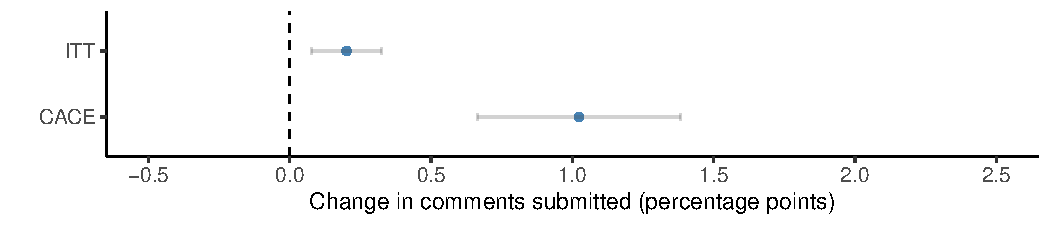
\includegraphics[width = \textwidth]{../figs/fg1.pdf}
\caption{Intent-to-treat effect and complier average causal effect, all cities}
\vspace{-0.5cm}
{\small \textit{Note: Tabular results can be found in \autoref{tab: itt} and \autoref{tab: cace}}}
\label{tab: treatment_placebo}
\end{figure}

CACEs for individual council meetings can be found in \autoref{fig: meta}, which also contains meta-analytic estimates of the aggregate CACE.\footnote{Precise null results in the Santa Monica pilot, Manhattan Beach, and Sierra Madre likely stem from small sample size. The Santa Monica pilot contained 91 opened emails (i.e., compliers), Manhattan Beach contained 70, and Sierra Madre contained 31. As 1 comment was submitted per 109 treated compliers across all cities, it is not unexpected to receive no comments in these cities.}  \autoref{fig: meta} also contains  estimates from three pilot studies, increasing the sample size to over 27,000 households. The point estimate using fixed effects meta-analysis including the pilot studies is 0.78 [95\% CI 0.51, 1.06], and excluding the pilot studies is 0.91 [95\% CI 0.56, 1.25] (see \autoref{fig: meta_nopilot}).

\begin{figure}[H]
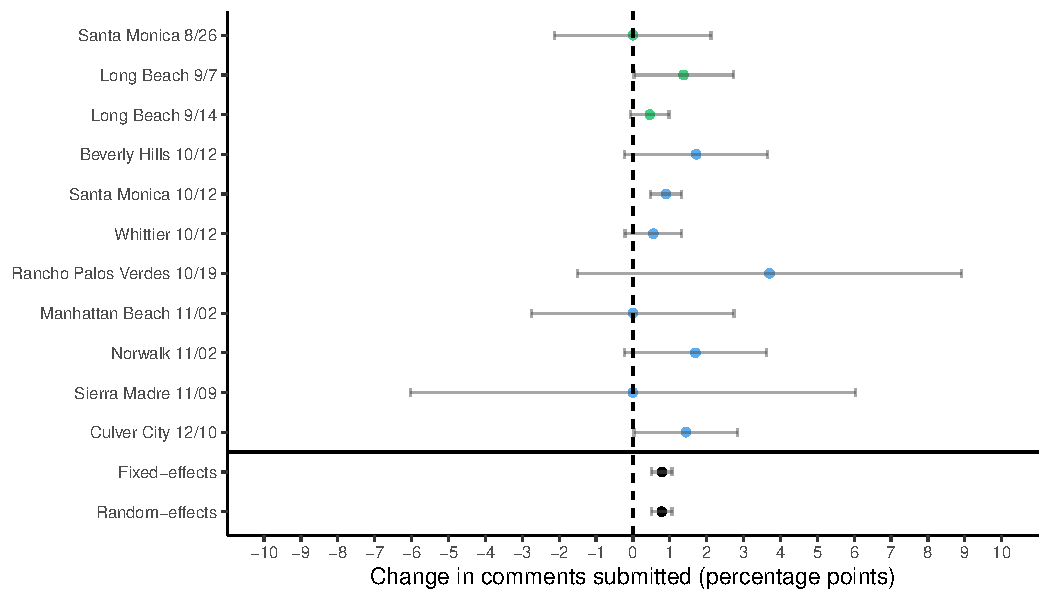
\includegraphics[width = \textwidth]{../figs/fg2.pdf}
\caption{Meta-analysis of complier average causal effects, by council meeting}
\vspace{-0.5cm}
{\small \textit{Note: Pilot studies in green. Tabular results can be found in \autoref{city_cace} and \autoref{meta}.}}
\label{fig: meta}
\end{figure}


\subsection{By treatment group}\label{sec: results_group}

In line with pre-registered hypotheses, \autoref{fig: all_treatments} shows that highlighting the costs of abstention (T3) had the largest effect on turnout (CACE = 1.44pp; RI p = 0.011; 95\% CI [0.73, 2.15]), priming economic self interest (T2) was the second most effective (CACE = 1.01pp; RI p = 0.071; 95\% CI [0.39, 1.63]), and the instructions-only treatment (T1) was the least effective (CACE = 0.54pp; RI p = 0.386; 95\% CI [0.06, 1.03]).\footnote{ITT randomization inference p-values are: 0.380 for T1, 0.089 for T2, and 0.039 for T3.} This translates to 1 comment per 67 emails opened in T3, 1 per 96 in T2, and 1 per 201 in T1. T3 and T1 are significantly different from each other at the 5\% level based on randomization inference and two-tailed linear hypothesis tests, while T2 and T1 are significantly different from each other at the 10\% level based on one-tailed tests (see \autoref{tab: linearhyp} and \autoref{tab: ri}).\footnote{A one-tailed test may be justified due to pre-registration of the relative magnitudes of effect sizes.} When grouped together, T2 and T3 are significantly different from T1 at the 5\% level using both randomization inference and a two-tailed linear hypothesis test. 

\begin{figure}[H]
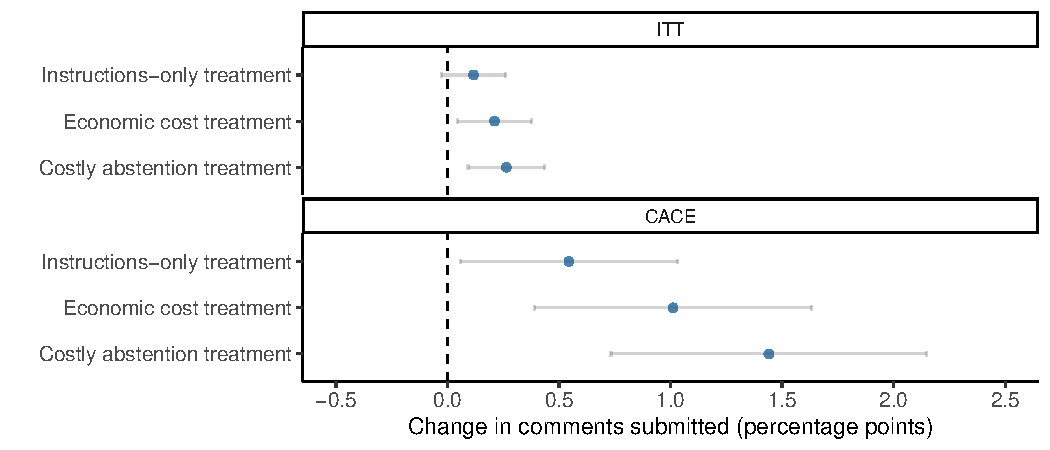
\includegraphics[width = \textwidth]{../figs/fg3.pdf}
\caption{Effects by treatment group, all cities}
\vspace{-0.5cm}
{\small \textit{Note: Tabular results can be found in \autoref{tab: itt} and \autoref{tab: cace}}}
\label{fig: all_treatments}
\end{figure}

To further asses confidence the costly abstention treatment was most effective, I fit a Bayesian linear multilevel model using prior distributions from my pre-registration power analysis,\footnote{Coefficient estimates and posterior distributions can be found in \autoref{fig: bayes_coef}. \autoref{fig: posterior_dists} depicts the posterior distributions of each coefficient and the differences between each coefficient.} and compute Bayes factors\footnote{The ratio of the likelihood of one particular hypothesis to the likelihood of another hypothesis.} for hypotheses that the differences between treatments are greater than zero. This analysis suggests that the costly abstention treatment is 5 times as likely to be larger than the economic cost treatment than not, and 97 times as likely to be larger than the instructions only treatment than not. 

These results align with the pre-registered \hyperref[theory: treatments]{theoretical predictions}. Providing instructions of how to participate increased participation, but only marginally. Priming economic concerns appears to be more effective than lowering participation costs alone. The strongest evidence supports the theory that highlighting costs of abstention is more effective than lowering attendance costs alone. Additionally, the collective strength of the economic cost and costly abstention treatments compared to the instructions-only treatment imply that economic or psychological motivators are more effective at driving participation than providing instructions or a clickable link alone. 

\subsection{Heterogeneous treatment effects}

I find suggestive evidence that turnout in local elections is associated with a sizable increase in the likelihood of making a public comment. Voters were both more likely to open the emails (see \autoref{tab: covs_compliance}) and 1.4pp more likely to comment than non-voters (see \autoref{fig: voting_cates}, RI p = 0.06).\footnote{The uncertainty of the estimates are a result of low turnout (9.4\% amongst the sample population)} There is therefore suggestive evidence that participation in local politics in the form of voting begets willingness to participate in other forms. Further research is necessary to uncover the mechanisms behind this finding. It is possible that missing an opportunity to have one’s voice heard may feel particularly costly for renters who already make the effort to participate in low-turnout municipal elections. Alternatively, renters who vote in local elections may already have a strong interest in local development, making them more responsive to treatment due to pre-existing interest in housing policy. 

\begin{figure}[H]
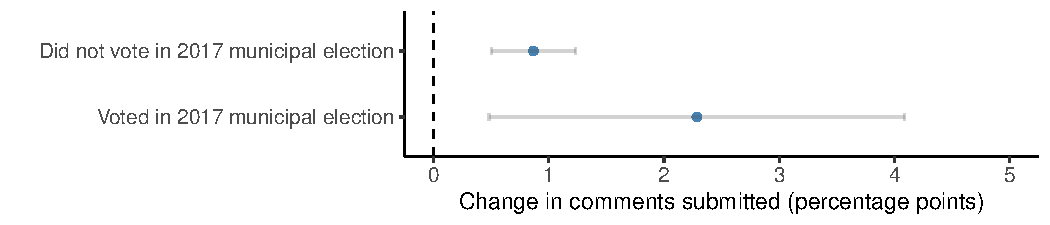
\includegraphics[width = \textwidth]{../figs/fg4.pdf}
\caption{Complier average causal effects by turnout}
\vspace{-0.5cm}
{\small \textit{Note: Tabular results can be found in \autoref{tab: cate}.}}
\label{fig: voting_cates}
\end{figure}

\subsection{Comment contents}\label{sec:how}

I examine the content of each comment to determine if individuals submitted: spoken or written comments, custom comments or used the pre-written comment supplied in the emails, and pro or anti-housing comments (see \autoref{fig: pro_anti_custom}). The vast majority of individuals (93\%) submitted written public comments, and the effect for spoken comments is only significant at the 10\% level. However, even written submissions were not purely costless. While the majority of written comments used the sample message included in the email, 29\% represented custom, personal comments. Many of these custom comments were deeply personal and reflected individuals' lived experiences with high housing costs.\footnote{I do not provide quotes of custom experimentally-induced comments as I did not ask for consent to re-print individuals' public comments.} For example, some discussed near experiences with homelessness, senior commenters discussed fear of being priced out of subsidized senior housing, and young renters lamented their inability to purchase a home like their parents. While some anti-housing comments were submitted, they represented only 4\% of total comments, and never comprised a majority of experimentally-induced comments in any council meetings.

\begin{figure}[H]
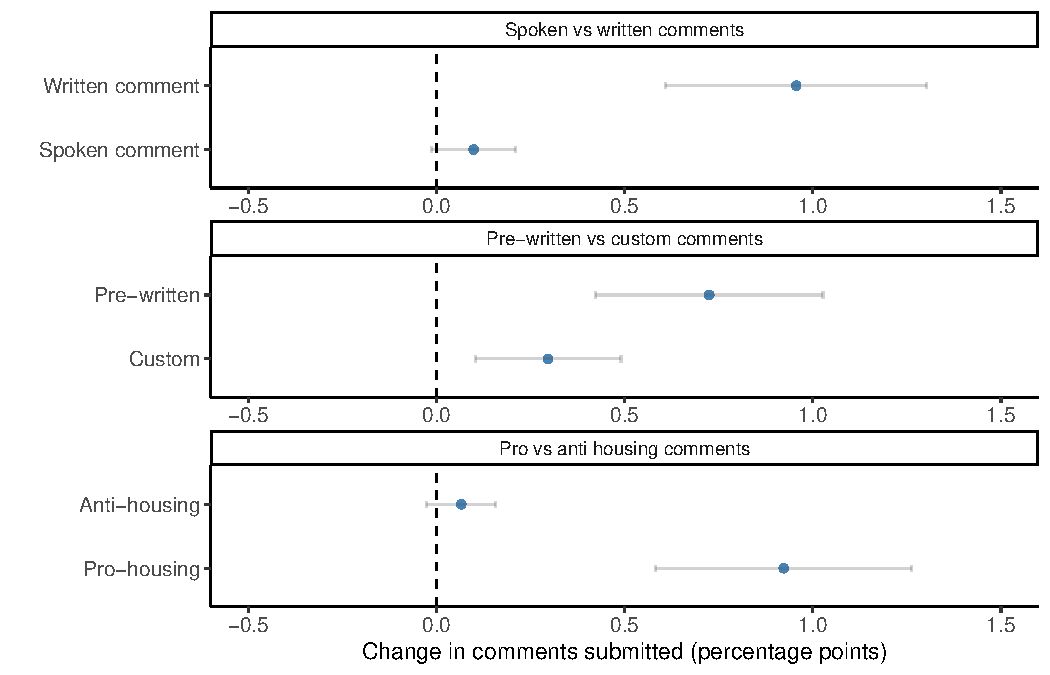
\includegraphics[width = \textwidth]{../figs/fg5.pdf}
\caption{CACE by type of comment}
\vspace{-0.5cm}
{\small \textit{Note: Tabular results can be found in \autoref{tab: disc}.}}
\label{fig: pro_anti_custom}
\end{figure}


\subsection{Substantive impact of comments and changes in representation}

I also investigate the substantive impact of the campaigns on each council meeting. \autoref{tab: comments_by_meeting} shows that the treatments meaningfully changed the quantity and composition of comments. Comments by treated individuals represented 8\% of total written public comments across all meetings, and 46\% of all pro-housing comments. Treatment-induced comments swung the balance of pro-versus-anti housing comments toward a more equal footing, altering the imbalances of comment makeup highlighted by \citet{yoder2020does} that were not changed merely by moving to an online setting \citep{einstein2021zoom}. The treatments therefore caused the makeup of council meeting comments to be more reflective of the broader public where remote access alone did not.

\begin{table}[H]
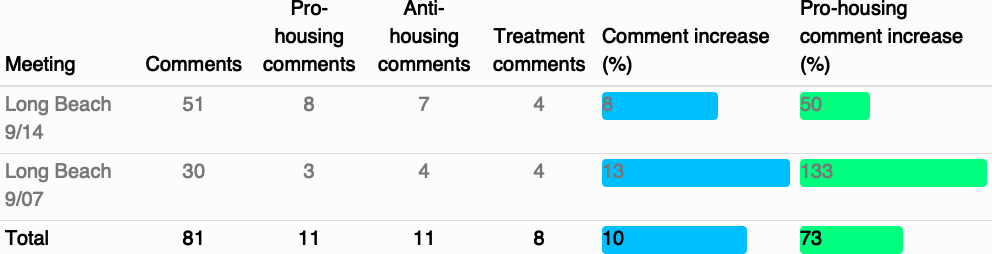
\includegraphics[width = \textwidth]{../tables/tbl1.png}
\caption{Examination of public comments in treated council meetings}
\label{tab: comments_by_meeting}
\end{table}
\vspace{-0.2cm}


These large effects of contact on overall turnout contrast sharply with, e.g., GOTV.\footnote{The cost-effectiveness of the campaign also contrasts sharply with GOTV. Comments were generated at a cost of \$4.80 per comment, compared with over \$450 per vote in GOTV Facebook campaigns and \$37 per vote in the most effective text messaging campaigns \citep{green2019get}.} In voter turnout settings, the large number of individuals who regularly vote makes the change in overall turnout due to campaigns relatively small. By contrast, even a few new participants in city council meetings can meaningfully change the composition of comments due to low equilibrium participation rates. Council members in observed meetings also alluded directly to the overall makeup of public comments when discussing and voting on issue items, implying that they are aware of the tenor of comments. 

\section{Conclusion}

Understanding how to motivate individuals to engage in personally costly collective action when gains from mobilization are long-term and uncertain is an enduring question in political economy. Homeowners with direct financial payoffs participate in local politics at disproportionately high rates. However, there is little evidence to suggest how to motivate those such as renters---who face long-term and uncertain payoffs---to participate.

I contribute to our understanding of how to motivate underrepresented groups to engage in costly political behavior using 8 email-outreach field experiments encouraging renters to participate in local politics in the form of commenting at city council meetings. In addition, I document how these  campaigns changed the balance of participation in civic bodies. Three treatment arms tested the effectiveness of messages that: (1) lowered the costs of participation only, (2) primed economic self-interest, or (3) highlighted the costs of abstention. Receipt of any treatment increased public comments by 1pp, while highlighting the cost of abstention increased comments by 1.4pp.  Individuals already engaged in local politics were more responsive to treatment. Treatment-induced comments represented 8\% of total comments and 46\% of pro-housing comments across all city council meetings. The treatments therefore overcame many of the traditional barriers to renter collective action, and changed the representation of civic bodies to be more reflective of the broader public. 

The results support the following theoretical and substantive conclusions. First, unlike voting, email can effectively increase political participation when participation can also be conducted remotely, particularly amongst those already engaged in politics. Second, low-cost outreach strategies can meaningfully increase political participation in low-turnout and lesser-known settings such as city council meetings. Third, outreach can change the representation of civic bodies to be more reflective of the broader public where increases in accessibility alone---such as online access---do not. Fourth, informational outreach alone is not particularly effective, but increasing perceived costs of abstention appears to be an effective motivator of collective action.

\clearpage
\pagebreak

\singlespace
\pdfbookmark[1]{References}{References}
\bibliography{bibliography}

\singlespace
\newpage
\appendix
\addcontentsline{toc}{section}{Appendix} % Add the appendix text to the document TOC
\part{\Large{Supporting Information}}% Start the appendix part
\parttoc 
%\section{Appendix}

\setcounter{table}{0}
\renewcommand{\thetable}{A\arabic{table}}
\setcounter{figure}{0}
\renewcommand{\thefigure}{A\arabic{figure}}
\pagenumbering{arabic}% resets `page` counter to 1
\renewcommand*{\thepage}{A\arabic{page}}

\normalsize
\newpage
\doublespace

\subsection{Housing net worth} \label{sec: theory}

\begin{figure}[H]
\begin{center}
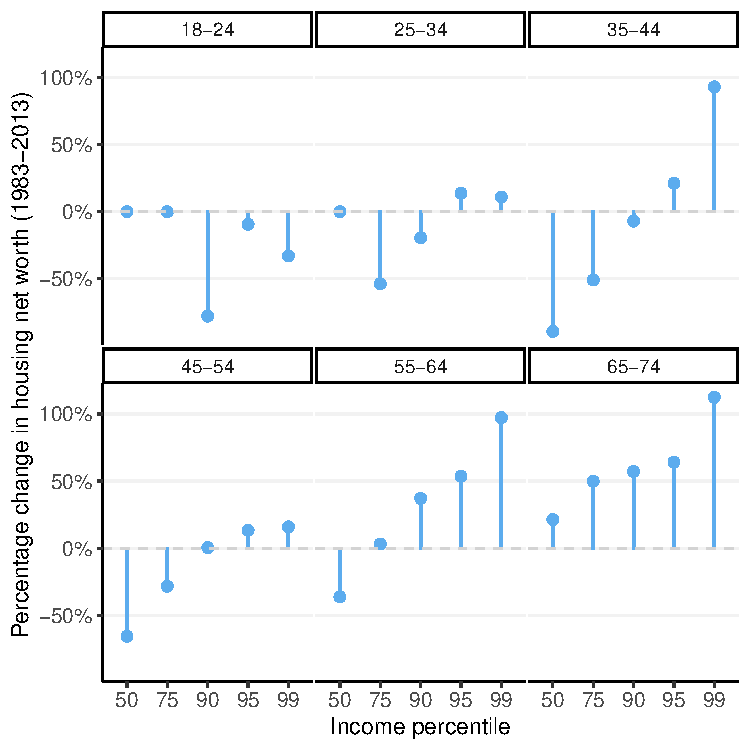
\includegraphics[width = 0.8\textwidth]{../figs/fgA1.pdf}
\caption{Change in housing net worth by age and income percentile}
\label{fig: housing_net_worth}
\end{center}
\vspace{-0.75cm}
Source: \citet{glaeser2018economic}
\end{figure}

\clearpage
\subsection{Voter file descriptive statistics} \label{sec: vf_desc}

\begin{table}[H]

\centering
\resizebox{\linewidth}{!}{
\begin{tabular}[t]{lrrrrrr}
\toprule
\multicolumn{1}{c}{ } & \multicolumn{2}{c}{Confirmed renter (N=641184)} & \multicolumn{2}{c}{Not confirmed renter (N=5045990)} & \multicolumn{2}{c}{ } \\
\cmidrule(l{3pt}r{3pt}){2-3} \cmidrule(l{3pt}r{3pt}){4-5}
  & Mean & Std. Dev. & Mean & Std. Dev. & Diff. in Means & p\\
\midrule
\cellcolor[HTML]{D3D3D3}{Email} & \cellcolor[HTML]{D3D3D3}{0.41} & \cellcolor[HTML]{D3D3D3}{0.49} & \cellcolor[HTML]{D3D3D3}{0.34} & \cellcolor[HTML]{D3D3D3}{0.48} & \cellcolor[HTML]{D3D3D3}{-0.07} & \cellcolor[HTML]{D3D3D3}{$<$0.01}\\
Phone & 0.52 & 0.50 & 0.52 & 0.50 & 0.00 & $<$0.01\\
\cellcolor[HTML]{D3D3D3}{Age} & \cellcolor[HTML]{D3D3D3}{43.39} & \cellcolor[HTML]{D3D3D3}{17.70} & \cellcolor[HTML]{D3D3D3}{47.84} & \cellcolor[HTML]{D3D3D3}{18.90} & \cellcolor[HTML]{D3D3D3}{4.46} & \cellcolor[HTML]{D3D3D3}{$<$0.01}\\
Years registered & 3.98 & 6.53 & 6.29 & 9.82 & 2.31 & $<$0.01\\
\cellcolor[HTML]{D3D3D3}{Female} & \cellcolor[HTML]{D3D3D3}{0.54} & \cellcolor[HTML]{D3D3D3}{0.50} & \cellcolor[HTML]{D3D3D3}{0.53} & \cellcolor[HTML]{D3D3D3}{0.50} & \cellcolor[HTML]{D3D3D3}{-0.01} & \cellcolor[HTML]{D3D3D3}{$<$0.01}\\
Speak English & 0.93 & 0.25 & 0.94 & 0.24 & 0.00 & $<$0.01\\
\cellcolor[HTML]{D3D3D3}{CA native} & \cellcolor[HTML]{D3D3D3}{0.48} & \cellcolor[HTML]{D3D3D3}{0.50} & \cellcolor[HTML]{D3D3D3}{0.54} & \cellcolor[HTML]{D3D3D3}{0.50} & \cellcolor[HTML]{D3D3D3}{0.07} & \cellcolor[HTML]{D3D3D3}{$<$0.01}\\
Democrat & 0.57 & 0.49 & 0.52 & 0.50 & -0.05 & $<$0.01\\
\cellcolor[HTML]{D3D3D3}{Republican} & \cellcolor[HTML]{D3D3D3}{0.11} & \cellcolor[HTML]{D3D3D3}{0.31} & \cellcolor[HTML]{D3D3D3}{0.18} & \cellcolor[HTML]{D3D3D3}{0.38} & \cellcolor[HTML]{D3D3D3}{0.07} & \cellcolor[HTML]{D3D3D3}{$<$0.01}\\
Independent & 0.25 & 0.43 & 0.24 & 0.43 & -0.01 & $<$0.01\\
\cellcolor[HTML]{D3D3D3}{Voted in 2020 general election} & \cellcolor[HTML]{D3D3D3}{0.69} & \cellcolor[HTML]{D3D3D3}{0.46} & \cellcolor[HTML]{D3D3D3}{0.74} & \cellcolor[HTML]{D3D3D3}{0.44} & \cellcolor[HTML]{D3D3D3}{0.05} & \cellcolor[HTML]{D3D3D3}{$<$0.01}\\
Voted in 2017 municipal election & 0.10 & 0.30 & 0.14 & 0.35 & 0.04 & $<$0.01\\
\cellcolor[HTML]{D3D3D3}{Voted in 2016 general election} & \cellcolor[HTML]{D3D3D3}{0.43} & \cellcolor[HTML]{D3D3D3}{0.49} & \cellcolor[HTML]{D3D3D3}{0.53} & \cellcolor[HTML]{D3D3D3}{0.50} & \cellcolor[HTML]{D3D3D3}{0.10} & \cellcolor[HTML]{D3D3D3}{$<$0.01}\\
\bottomrule
\end{tabular}}
\caption{Balance table: confirmed renters vs. non-confirmed renters}
\end{table}

\begin{table}[H]

\centering
\resizebox{\linewidth}{!}{
\begin{tabular}[t]{lrrrrrr}
\toprule
\multicolumn{1}{c}{ } & \multicolumn{2}{c}{Email listed (N=266057)} & \multicolumn{2}{c}{Email not listed (N=375127)} & \multicolumn{2}{c}{ } \\
\cmidrule(l{3pt}r{3pt}){2-3} \cmidrule(l{3pt}r{3pt}){4-5}
  & Mean & Std. Dev. & Mean & Std. Dev. & Diff. in Means & p\\
\midrule
\cellcolor[HTML]{D3D3D3}{Phone} & \cellcolor[HTML]{D3D3D3}{0.80} & \cellcolor[HTML]{D3D3D3}{0.40} & \cellcolor[HTML]{D3D3D3}{0.32} & \cellcolor[HTML]{D3D3D3}{0.47} & \cellcolor[HTML]{D3D3D3}{-0.48} & \cellcolor[HTML]{D3D3D3}{$<$0.01}\\
Age & 38.43 & 14.75 & 46.91 & 18.75 & 8.48 & $<$0.01\\
\cellcolor[HTML]{D3D3D3}{Years registered} & \cellcolor[HTML]{D3D3D3}{1.87} & \cellcolor[HTML]{D3D3D3}{2.99} & \cellcolor[HTML]{D3D3D3}{5.47} & \cellcolor[HTML]{D3D3D3}{7.83} & \cellcolor[HTML]{D3D3D3}{3.59} & \cellcolor[HTML]{D3D3D3}{$<$0.01}\\
Female & 0.53 & 0.50 & 0.54 & 0.50 & 0.01 & $<$0.01\\
\cellcolor[HTML]{D3D3D3}{Speak English} & \cellcolor[HTML]{D3D3D3}{0.96} & \cellcolor[HTML]{D3D3D3}{0.20} & \cellcolor[HTML]{D3D3D3}{0.92} & \cellcolor[HTML]{D3D3D3}{0.28} & \cellcolor[HTML]{D3D3D3}{-0.04} & \cellcolor[HTML]{D3D3D3}{$<$0.01}\\
CA native & 0.52 & 0.50 & 0.44 & 0.50 & -0.08 & $<$0.01\\
\cellcolor[HTML]{D3D3D3}{Year building constructed} & \cellcolor[HTML]{D3D3D3}{1967.48} & \cellcolor[HTML]{D3D3D3}{21.55} & \cellcolor[HTML]{D3D3D3}{1966.61} & \cellcolor[HTML]{D3D3D3}{20.93} & \cellcolor[HTML]{D3D3D3}{-0.87} & \cellcolor[HTML]{D3D3D3}{$<$0.01}\\
Units in building & 43.41 & 66.82 & 40.60 & 61.00 & -2.81 & $<$0.01\\
\cellcolor[HTML]{D3D3D3}{Democrat} & \cellcolor[HTML]{D3D3D3}{0.59} & \cellcolor[HTML]{D3D3D3}{0.49} & \cellcolor[HTML]{D3D3D3}{0.56} & \cellcolor[HTML]{D3D3D3}{0.50} & \cellcolor[HTML]{D3D3D3}{-0.04} & \cellcolor[HTML]{D3D3D3}{$<$0.01}\\
Republican & 0.10 & 0.30 & 0.11 & 0.32 & 0.01 & $<$0.01\\
\cellcolor[HTML]{D3D3D3}{Independent} & \cellcolor[HTML]{D3D3D3}{0.24} & \cellcolor[HTML]{D3D3D3}{0.43} & \cellcolor[HTML]{D3D3D3}{0.26} & \cellcolor[HTML]{D3D3D3}{0.44} & \cellcolor[HTML]{D3D3D3}{0.02} & \cellcolor[HTML]{D3D3D3}{$<$0.01}\\
Voted in 2020 general election & 0.77 & 0.42 & 0.63 & 0.48 & -0.13 & $<$0.01\\
\cellcolor[HTML]{D3D3D3}{Voted in 2017 municipal election} & \cellcolor[HTML]{D3D3D3}{0.09} & \cellcolor[HTML]{D3D3D3}{0.29} & \cellcolor[HTML]{D3D3D3}{0.11} & \cellcolor[HTML]{D3D3D3}{0.31} & \cellcolor[HTML]{D3D3D3}{0.02} & \cellcolor[HTML]{D3D3D3}{$<$0.01}\\
Voted in 2016 general election & 0.40 & 0.49 & 0.45 & 0.50 & 0.05 & $<$0.01\\
\bottomrule
\end{tabular}}
\caption{Balance table: renters with emails listed in voter file vs. those without}
\end{table}


\subsection{Treatment messages} \label{sec: messages}

\vspace{-0.75cm}
\begin{figure}[H]
    \centering
        \begin{subfigure}[t]{0.45\textwidth}
        \centering
        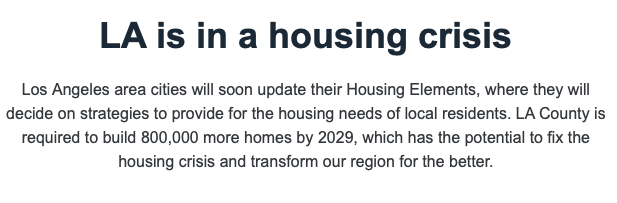
\includegraphics[width=5.5cm]{../figs/fgA2.1.png}
        \caption{Placebo treatment message} \label{subfig: placebo}
    \end{subfigure}
    ~
    \begin{subfigure}[t]{0.45\textwidth}
        \centering
        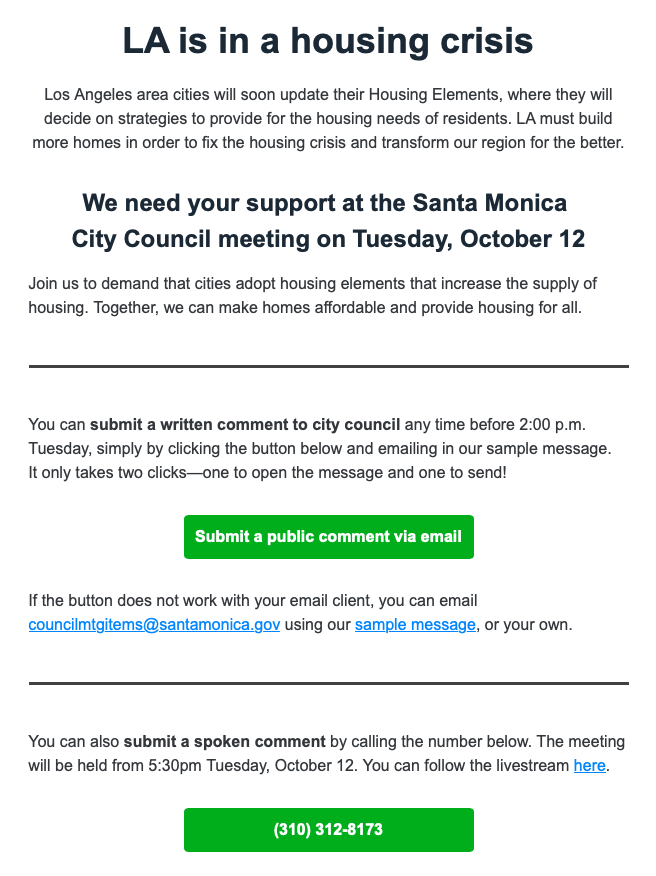
\includegraphics[width=5.5cm]{../figs/fgA2.2.png}
        \caption{Instructions only treatment message} \label{subfig: T1}
        \vspace{0.5cm}
    \end{subfigure}
    ~ 
    \begin{subfigure}[b]{0.45\textwidth}
        \centering
        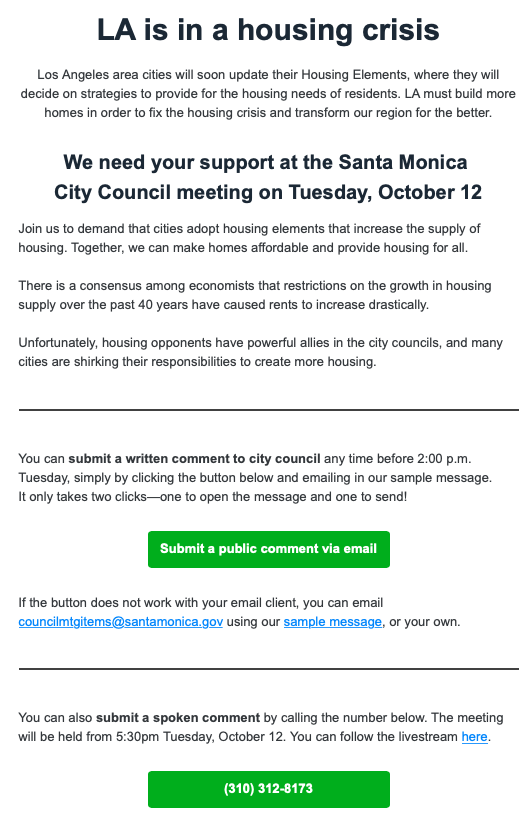
\includegraphics[width=5.5cm]{../figs/fgA2.3.png}
        \caption{Economic treatment message} \label{subfig: T2}
    \end{subfigure}
    ~
    \begin{subfigure}[b]{0.45\textwidth}
        \centering
        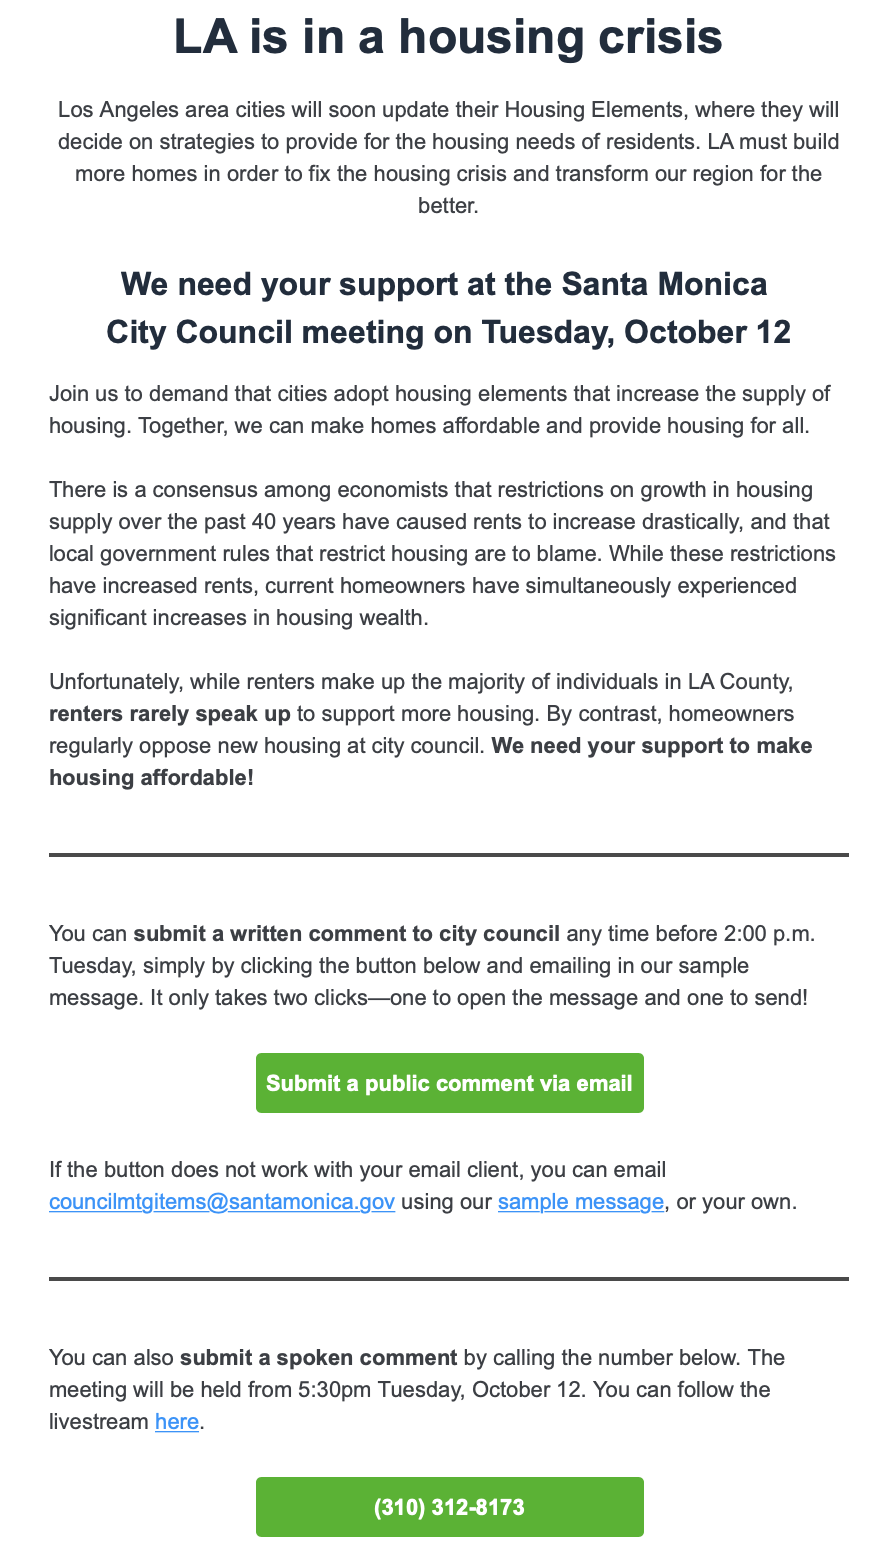
\includegraphics[width=5.5cm]{../figs/fgA2.4.png}
        \caption{Costly abstention treatment message} \label{subfig: T3}
    \end{subfigure}
    ~
    \caption{Example treatments and wording (Santa Monica experiment)}\label{fig: treatments}
\end{figure}


\subsection{Treatment details} \label{sec: treatment_details}

\begin{figure}[H]
\hspace*{-3.5cm} 
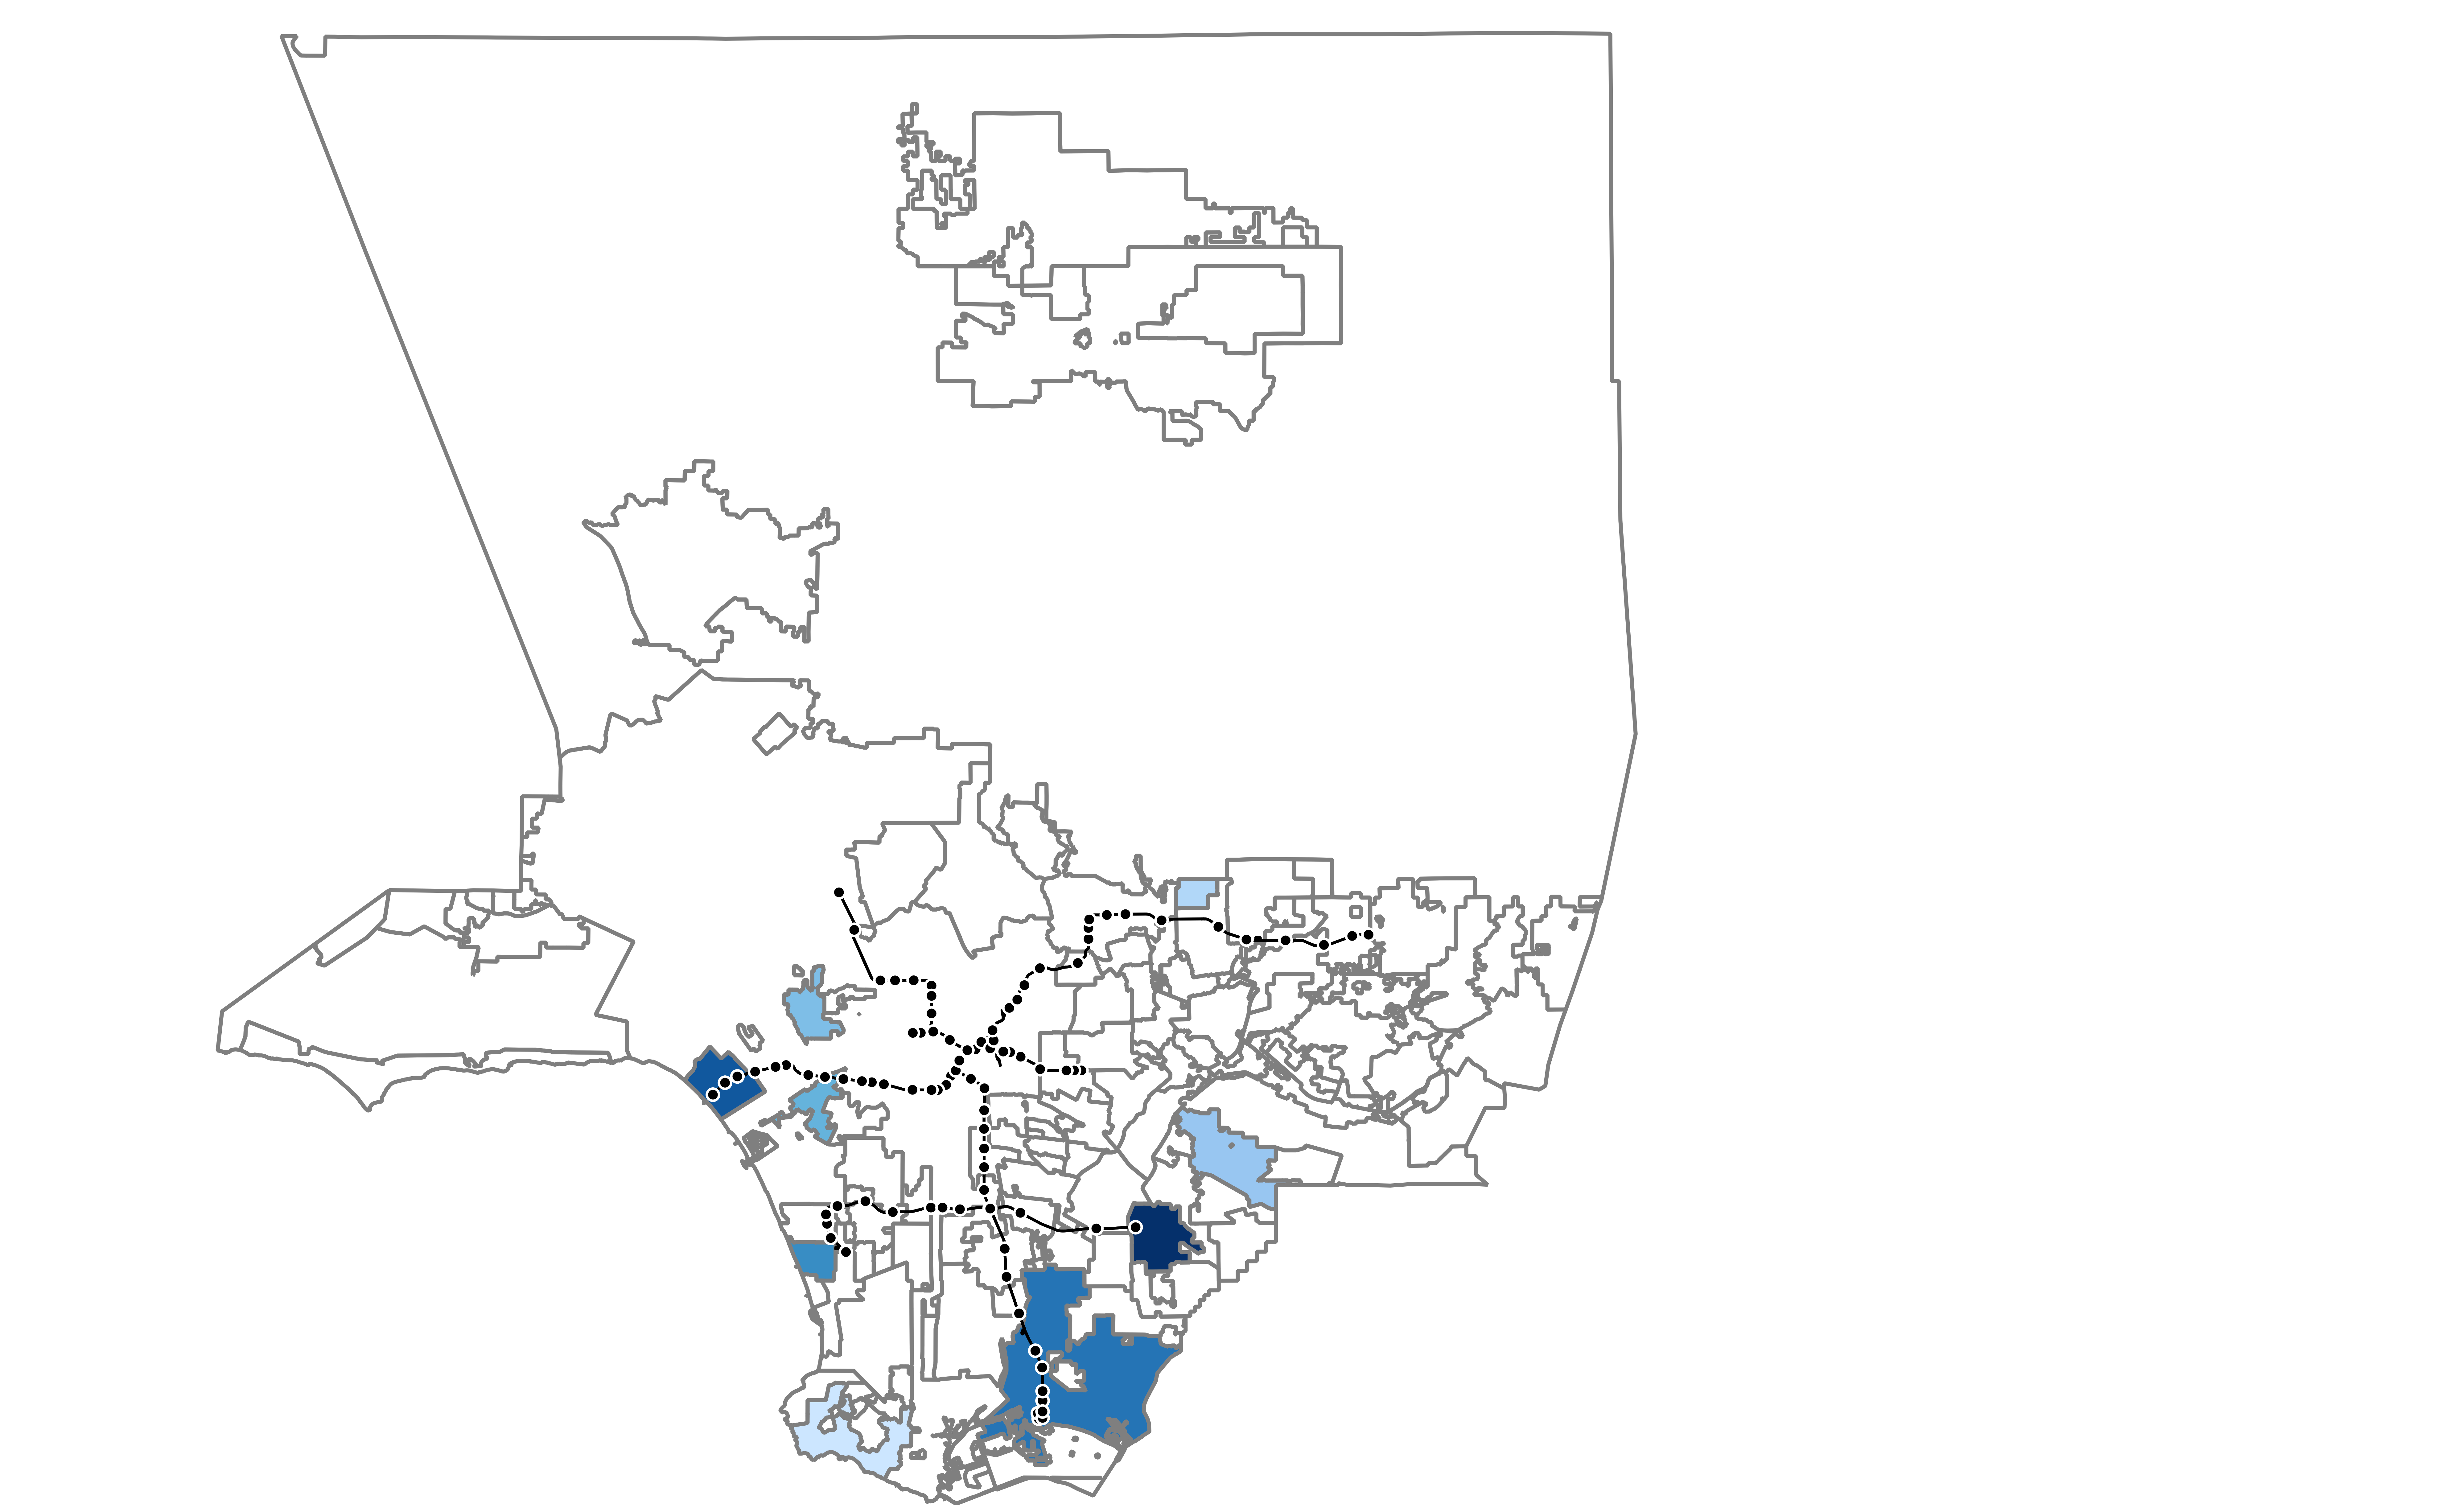
\includegraphics[width = 30cm]{../figs/fgA5.png}
\caption{Map of cities in Los Angeles county by experiment status}
\label{fig: map_treated_cities}
\vspace{-0.5cm}
\begin{singlespace}
\textit{Note:} Cities in which an experiment was launched in blue.  Cities shaded by population density. Los Angeles Metro rail lines and rail stations in black. 
\end{singlespace}
\end{figure}


\pagebreak
\subsubsection{Sample comment} \label{sec: sample_comment}
\noindent
Subject: \\
\noindent
Public comment for [DATE] council meeting agenda item [ITEM NUMBER] \\

\noindent
Body: \\
\noindent
Dear City Council, \\

\noindent
I’m writing to express my concern about our affordable housing shortage and its impact on the future of our city. Exclusionary zoning and land use practices have led to an undersupply of affordable medium- and high-density housing near jobs and transit, and have perpetuated segregated living patterns and the exclusion of historically disadvantaged communities. \\

\noindent
[CITY] has an opportunity to address the need for more housing in a way that furthers equity, environmental sustainability, and economic recovery in its housing element update. We should update the housing element in a way that encourages historically high housing growth, while furthering fair housing opportunities and undoing patterns of discrimination in housing. We can’t miss this opportunity to fix our city’s housing crisis. \\

\noindent
I urge you to legalize more housing, make housing easier to build, fund affordable housing and end homelessness, and strengthen tenants’ rights. \\

\noindent
Sincerely, \\
\noindent
FIRSTNAME LASTNAME

\pagebreak
\subsection{Ethics} \label{sec: ethics}

Any intervention motivating individuals to change their behavior should be held to high ethical standards, particularly when the intervention involves participation in and effects on governmental processes. Beyond IRB approval, I argue this project falls within ethical bounds for the reasons outlined below. 

First, these messaging campaigns are commonly conducted by political campaigns and nonprofit organizations, and individuals in the voter file therefore would have received messages with or without researcher randomization and measurement. 

Second, the interventions are designed to minimize a pre-existing imbalance in representation by increasing representation amongst a historically underrepresented group. Treatments are designed to encourage renters to participate (albeit not coercively) and make local governance more reflective of the general population.  

Third, the interventions do not directly effect electoral outcomes (as highlighted by \citet{slough2019ethics} and \citet{mcdermott2020ethics}). I recognize that local officials may change their votes based on perceived changes in support levels that the experiment might cause. However, ultimate decisions and votes still rest with local elected officials. 

Fourth, the interventions focus on increasing the supply of housing generally across the LA region, not on particular developments or neighborhoods. Treatment and sample messages also specifically encourage individuals to advocate for \textit{affordable} (i.e., government subsidized) housing developments. We should therefore expect the targeted groups to benefit from the research through decreased rents and increased access to affordable housing. 

Fifth, in social-welfare enhancing interventions such as ``green nudges,'' \citet{bovens2009ethics} and \citet{schubert2017green} argue that it should be possible ``for everyone who is watchful to unmask the manipulation.'' The interventions meet this criteria, as the messages come from an advocacy group that is transparent in their motivations.

While informed consent was not received from individuals prior to treatment, the research is: (1) minimal risk compared to similar outreach emails that individuals who listed their email addresses in the voter file would otherwise receive without researcher measurement, (2) permission to obtain the voter file and conduct the research was obtained from the Los Angeles County Registrar in addition to a university IRB, (3) individuals would have received similar messages from advocacy organizations with or without researcher measurement, (4) treatment messages noted that they were part of a ``collaboration between Abundant Housing Los Angeles and academic researchers at [redacted for peer review]'' and were transparent in motivation, and (5) participant behavior may have changed if subjects were aware they were part of an academic study. The only potential deception was therefore anonymized data collection for the purpose of measurement.  


\pagebreak
\subsection{Analytical procedure details} \label{sec: analytic_details}

By randomly assigning individuals to a \hyperref[subfig: placebo]{placebo control} with no mention of council meetings, but featuring the same subject line and preview text as the treatment emails, I am able to observe the outcomes of a random sample of compliers (email openers) in the placebo group. Email opens are monitored using software that detects whether an individual opens a message. Tests for differential compliance by treatment group and differential covariate predictiveness of compliance can be found in \autoref{fig: differential_compliance} and \autoref{tab: covs_compliance}.

For the primary estimand (i.e., the CACE), I estimate the OLS specifications below:

\vspace{-1cm}
\begin{equation}
  \tag{With \citet{lin2013agnostic} covariate adjustment}
  Y_i = \alpha + \beta_1Z_i + \beta_2 X_i^c + \gamma X_i^c Z_i + \delta_{city} +  \epsilon_i
  \label{eqn: cov}
\end{equation}

\vspace{-2cm}
\begin{equation}
  \tag{Without covariate adjustment}
  Y_i = \alpha + \beta_1Z_i + \delta_{city} + \epsilon_i
  \label{eqn: nocov}
\end{equation}

where  $Y_i$ is the individual-level comment outcome, $Z_i$ is an indicator for the treatment group, $X_i^c$  is a vector of pre-treatment covariates for unit $i$ that have been centered to have mean zero, and $\delta_{city}$ are city (block) fixed effects. 

The following pre-registered pre-treatment covariates are included in the regression specification: \textit{city, number of units in the building, gender, age, building age, primary language spoken, vote history, and party affiliation}. I show that these variables are balanced between the placebo and treatment groups in \nameref{sec: balance}. Missing covariates are mean imputed.

Randomization inference p-values for the ITT are calculated by simulating a large number of ``fake'' random assignments for all units using the same procedure as the real random assignment, and estimating a treatment effect for each fake random assignment. I then calculate a p value as the proportion of times fake treatment assignments resulted in an effect size larger than the actual treatment effect. For the CACE, I make the additional assumption that observed compliance would exist regardless of treatment status and hold compliers constant across simulations. I conduct 10,000 simulations for the CACE and 1000 simulations for the ITT. All simulations were performed without covariate adjustment due to high computational demands. For CATEs, I generate the full schedule of potential outcomes under the null hypothesis that the true treatment effect is constant and equal to the estimated CACE. Then, I simulate random assignment 10,000 times and calculate the proportion of instances the simulated estimate of the interaction effect is at least as large (in absolute value) as the actual estimate.

In the precision-weighted fixed effects meta-analysis, weights are equal to the inverse of the variance. For council meetings where no comments are reported in treatment or placebo, I estimate standard errors according to the procedure described in \citet{gelman2006data}. See p. 17, footnote 1: ``Consider a survey of size $n$ with $y$ Yes responses and $n-y$ No responses. The estimated proportion of the population who woul­d answer Yes to this survey is $\hat{p} = y/n$, and the standard error of this estimate is $\sqrt{\hat{p}(1-\hat{p})/n}$. This estimate and standard error are usually reasonable unless $y=0$ or $n-y = 0$, in which case the resulting standard error estimate of zero is misleading. A reasonable quick correction when $y$ or $n-y$ is near zero is to use the estimate $\hat{p} =(y+1)/(n+2)$ with standard error $\sqrt{\hat{p}(1-\hat{p})/n}$.''

Note that while replication code is available for the creation of the identified renter sample (i.e., merging the voter file with Los Angeles Department of City Planning records of multi-unit housing developments), the full voter file cannot be provided for both legal and ethical reasons. However, all data used in the analyses described in this section  are available in anonymized form. 


\pagebreak
\subsection{Balance} \label{sec: balance}

\begin{table}
\centering
\fontsize{10}{12}\selectfont
\resizebox{\linewidth}{!}{
\begin{tabular}[t]{lrrrrrr}
\toprule
\multicolumn{1}{c}{ } & \multicolumn{2}{c}{Placebo (N=2007)} & \multicolumn{2}{c}{Treatment (N=17944)} & \multicolumn{2}{c}{ } \\
\cmidrule(l{3pt}r{3pt}){2-3} \cmidrule(l{3pt}r{3pt}){4-5}
  & Mean & Std. Dev. & Mean & Std. Dev. & Diff. in Means & p\\
\midrule
\cellcolor[HTML]{D3D3D3}{Female} & \cellcolor[HTML]{D3D3D3}{0.52} & \cellcolor[HTML]{D3D3D3}{0.50} & \cellcolor[HTML]{D3D3D3}{0.53} & \cellcolor[HTML]{D3D3D3}{0.50} & \cellcolor[HTML]{D3D3D3}{0.02} & \cellcolor[HTML]{D3D3D3}{0.11}\\
Speak English & 0.98 & 0.12 & 0.98 & 0.14 & 0.00 & 0.27\\
\cellcolor[HTML]{D3D3D3}{Age} & \cellcolor[HTML]{D3D3D3}{41.60} & \cellcolor[HTML]{D3D3D3}{15.76} & \cellcolor[HTML]{D3D3D3}{41.25} & \cellcolor[HTML]{D3D3D3}{15.62} & \cellcolor[HTML]{D3D3D3}{-0.37} & \cellcolor[HTML]{D3D3D3}{0.31}\\
Year building constructed & 1964.93 & 18.63 & 1964.83 & 18.03 & -0.14 & 0.75\\
\cellcolor[HTML]{D3D3D3}{Units in building} & \cellcolor[HTML]{D3D3D3}{34.25} & \cellcolor[HTML]{D3D3D3}{64.90} & \cellcolor[HTML]{D3D3D3}{34.39} & \cellcolor[HTML]{D3D3D3}{66.40} & \cellcolor[HTML]{D3D3D3}{0.08} & \cellcolor[HTML]{D3D3D3}{0.96}\\
Democrat & 0.57 & 0.49 & 0.58 & 0.49 & 0.01 & 0.41\\
\cellcolor[HTML]{D3D3D3}{Republican} & \cellcolor[HTML]{D3D3D3}{0.13} & \cellcolor[HTML]{D3D3D3}{0.33} & \cellcolor[HTML]{D3D3D3}{0.11} & \cellcolor[HTML]{D3D3D3}{0.32} & \cellcolor[HTML]{D3D3D3}{-0.01} & \cellcolor[HTML]{D3D3D3}{0.21}\\
Independent & 0.24 & 0.43 & 0.24 & 0.43 & 0.00 & 0.73\\
\cellcolor[HTML]{D3D3D3}{Voted in 2020 general election} & \cellcolor[HTML]{D3D3D3}{0.79} & \cellcolor[HTML]{D3D3D3}{0.40} & \cellcolor[HTML]{D3D3D3}{0.81} & \cellcolor[HTML]{D3D3D3}{0.40} & \cellcolor[HTML]{D3D3D3}{0.01} & \cellcolor[HTML]{D3D3D3}{0.28}\\
Voted in 2017 municipal election & 0.10 & 0.30 & 0.09 & 0.29 & -0.01 & 0.28\\
\cellcolor[HTML]{D3D3D3}{Voted in 2016 general election} & \cellcolor[HTML]{D3D3D3}{0.45} & \cellcolor[HTML]{D3D3D3}{0.50} & \cellcolor[HTML]{D3D3D3}{0.44} & \cellcolor[HTML]{D3D3D3}{0.50} & \cellcolor[HTML]{D3D3D3}{0.00} & \cellcolor[HTML]{D3D3D3}{0.75}\\
\bottomrule
\end{tabular}}
\end{table}

\begin{table}[H]
\centering
\fontsize{10}{12}\selectfont
\resizebox{\linewidth}{!}{
\begin{tabular}[t]{lrrrrrrrr}
\toprule
\multicolumn{1}{c}{ } & \multicolumn{2}{c}{Placebo (N=2007)} & \multicolumn{2}{c}{Treatment 1 (N=5984)} & \multicolumn{2}{c}{Treatment 2 (N=6002)} & \multicolumn{2}{c}{Treatment 3 (N=5958)} \\
\cmidrule(l{3pt}r{3pt}){2-3} \cmidrule(l{3pt}r{3pt}){4-5} \cmidrule(l{3pt}r{3pt}){6-7} \cmidrule(l{3pt}r{3pt}){8-9}
  & Mean & Std. Dev. & Mean & Std. Dev. & Mean & Std. Dev. & Mean & Std. Dev.\\
\midrule
\cellcolor[HTML]{D3D3D3}{Female} & \cellcolor[HTML]{D3D3D3}{0.52} & \cellcolor[HTML]{D3D3D3}{0.50} & \cellcolor[HTML]{D3D3D3}{0.52} & \cellcolor[HTML]{D3D3D3}{0.50} & \cellcolor[HTML]{D3D3D3}{0.54} & \cellcolor[HTML]{D3D3D3}{0.50} & \cellcolor[HTML]{D3D3D3}{0.54} & \cellcolor[HTML]{D3D3D3}{0.50}\\
Speak English & 0.98 & 0.12 & 0.98 & 0.14 & 0.98 & 0.13 & 0.98 & 0.14\\
\cellcolor[HTML]{D3D3D3}{Age} & \cellcolor[HTML]{D3D3D3}{41.60} & \cellcolor[HTML]{D3D3D3}{15.76} & \cellcolor[HTML]{D3D3D3}{41.16} & \cellcolor[HTML]{D3D3D3}{15.61} & \cellcolor[HTML]{D3D3D3}{41.35} & \cellcolor[HTML]{D3D3D3}{15.63} & \cellcolor[HTML]{D3D3D3}{41.23} & \cellcolor[HTML]{D3D3D3}{15.62}\\
Year building constructed & 1964.93 & 18.63 & 1964.83 & 17.88 & 1964.83 & 18.33 & 1964.84 & 17.88\\
\cellcolor[HTML]{D3D3D3}{Units in building} & \cellcolor[HTML]{D3D3D3}{34.25} & \cellcolor[HTML]{D3D3D3}{64.90} & \cellcolor[HTML]{D3D3D3}{34.31} & \cellcolor[HTML]{D3D3D3}{66.10} & \cellcolor[HTML]{D3D3D3}{34.01} & \cellcolor[HTML]{D3D3D3}{66.54} & \cellcolor[HTML]{D3D3D3}{34.86} & \cellcolor[HTML]{D3D3D3}{66.56}\\
Democrat & 0.57 & 0.49 & 0.58 & 0.49 & 0.60 & 0.49 & 0.58 & 0.49\\
\cellcolor[HTML]{D3D3D3}{Republican} & \cellcolor[HTML]{D3D3D3}{0.13} & \cellcolor[HTML]{D3D3D3}{0.33} & \cellcolor[HTML]{D3D3D3}{0.11} & \cellcolor[HTML]{D3D3D3}{0.32} & \cellcolor[HTML]{D3D3D3}{0.11} & \cellcolor[HTML]{D3D3D3}{0.31} & \cellcolor[HTML]{D3D3D3}{0.12} & \cellcolor[HTML]{D3D3D3}{0.33}\\
Independent & 0.24 & 0.43 & 0.25 & 0.43 & 0.24 & 0.43 & 0.24 & 0.43\\
\cellcolor[HTML]{D3D3D3}{Voted in 2020 general election} & \cellcolor[HTML]{D3D3D3}{0.79} & \cellcolor[HTML]{D3D3D3}{0.40} & \cellcolor[HTML]{D3D3D3}{0.80} & \cellcolor[HTML]{D3D3D3}{0.40} & \cellcolor[HTML]{D3D3D3}{0.81} & \cellcolor[HTML]{D3D3D3}{0.40} & \cellcolor[HTML]{D3D3D3}{0.81} & \cellcolor[HTML]{D3D3D3}{0.39}\\
Voted in 2017 municipal election & 0.10 & 0.30 & 0.09 & 0.29 & 0.10 & 0.30 & 0.09 & 0.29\\
\cellcolor[HTML]{D3D3D3}{Voted in 2016 general election} & \cellcolor[HTML]{D3D3D3}{0.45} & \cellcolor[HTML]{D3D3D3}{0.50} & \cellcolor[HTML]{D3D3D3}{0.45} & \cellcolor[HTML]{D3D3D3}{0.50} & \cellcolor[HTML]{D3D3D3}{0.45} & \cellcolor[HTML]{D3D3D3}{0.50} & \cellcolor[HTML]{D3D3D3}{0.43} & \cellcolor[HTML]{D3D3D3}{0.50}\\
\bottomrule
\end{tabular}}
\caption{Covariate balance across all treatment groups}
\end{table}


\pagebreak
\subsection{Tests for differential compliance} \label{sec: diff_compliance}

\begin{figure}[H]
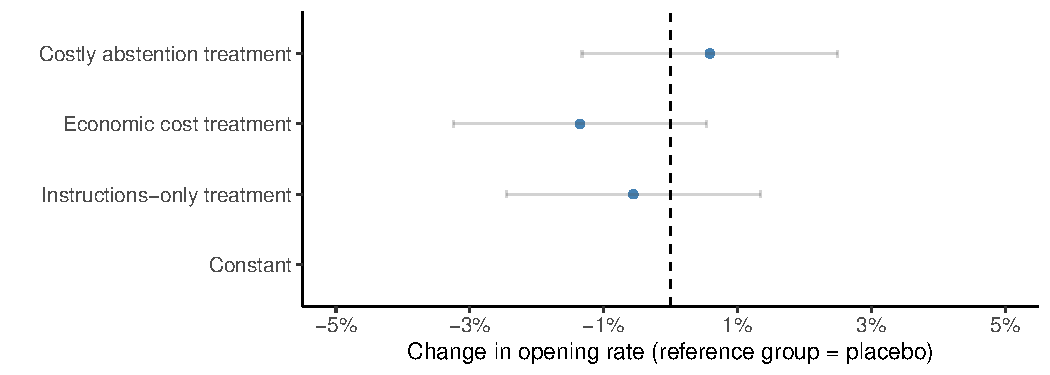
\includegraphics[width = \textwidth]{../figs/fgA4.pdf}
\caption{Average treatment effect on email opening, all cities}
\label{fig: differential_compliance}
\end{figure}

\begin{figure}[H]
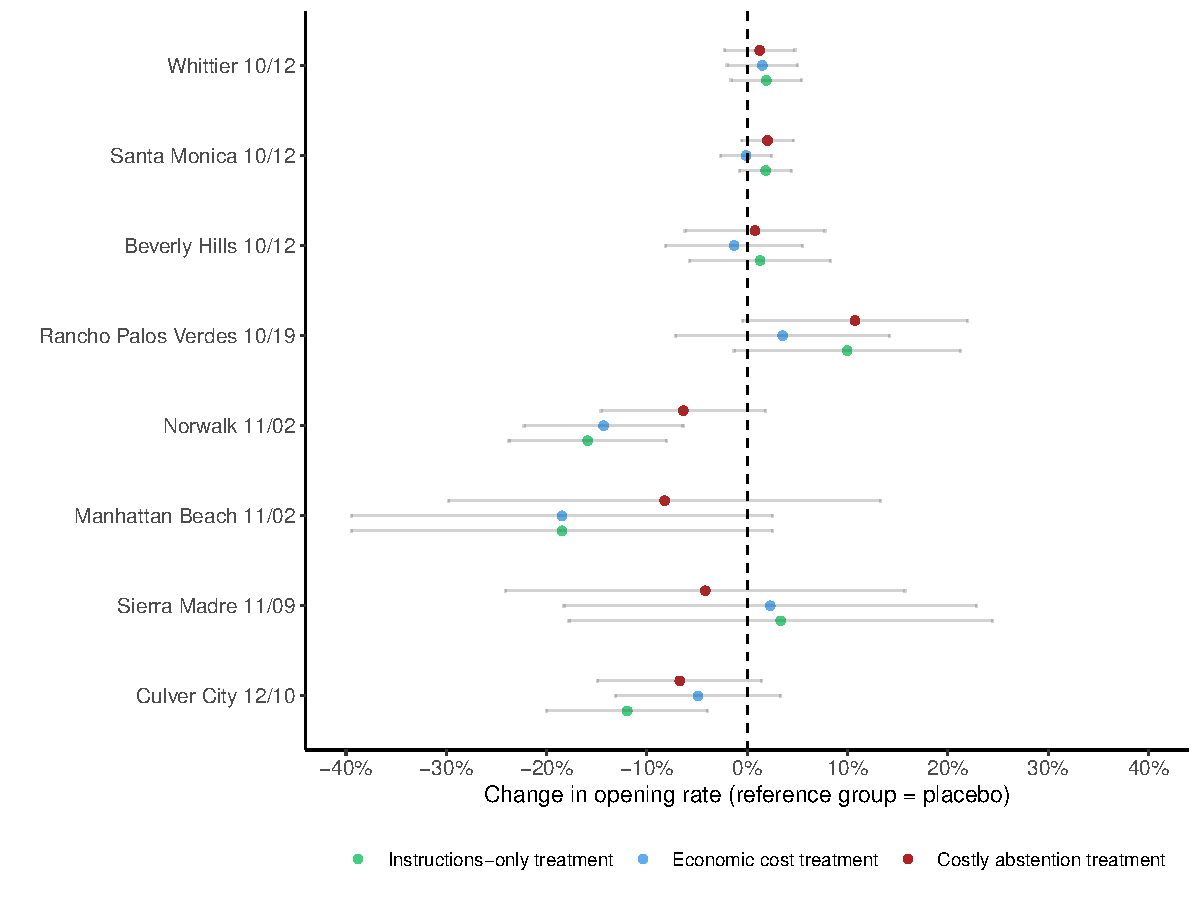
\includegraphics[width = \textwidth]{../figs/fgA5.pdf}
\caption{Average treatment effect on email opening, by city}
\label{fig: differential_compliance_city}
\end{figure}

\begin{table}
\centering
\begin{tabular}[t]{lcccc}
\toprule
  & Placebo & Treatment 1 & Treatment 2 & Treatment 3\\
\midrule
\cellcolor{gray!20}{Constant} & \cellcolor{gray!20}{\num{-0.321}} & \cellcolor{gray!20}{\num{-0.535}} & \cellcolor{gray!20}{\num{-0.565}} & \cellcolor{gray!20}{\num{0.216}}\\
 & (\num{0.980}) & (\num{0.569}) & (\num{0.560}) & (\num{0.563})\\
\cellcolor{gray!20}{Female} & \cellcolor{gray!20}{\num{-0.028}} & \cellcolor{gray!20}{\num{0.004}} & \cellcolor{gray!20}{\num{-0.012}} & \cellcolor{gray!20}{\num{-0.004}}\\
 & (\num{0.017}) & (\num{0.010}) & (\num{0.010}) & (\num{0.010})\\
\cellcolor{gray!20}{Speak English} & \cellcolor{gray!20}{\num{0.009}} & \cellcolor{gray!20}{\num{0.045}} & \cellcolor{gray!20}{\num{-0.020}} & \cellcolor{gray!20}{\num{-0.042}}\\
 & (\num{0.069}) & (\num{0.031}) & (\num{0.037}) & (\num{0.040})\\
\cellcolor{gray!20}{Age} & \cellcolor{gray!20}{\num{0.000}} & \cellcolor{gray!20}{\num{0.000}} & \cellcolor{gray!20}{\num{0.000}} & \cellcolor{gray!20}{\num{0.000}}\\
 & (\num{0.001}) & (\num{0.000}) & (\num{0.000}) & (\num{0.000})\\
\cellcolor{gray!20}{Year building constructed} & \cellcolor{gray!20}{\num{0.000}} & \cellcolor{gray!20}{\num{0.000}} & \cellcolor{gray!20}{\num{0.000}} & \cellcolor{gray!20}{\num{0.000}}\\
 & (\num{0.000}) & (\num{0.000}) & (\num{0.000}) & \vphantom{1} (\num{0.000})\\
\cellcolor{gray!20}{Units in building} & \cellcolor{gray!20}{\num{0.000}} & \cellcolor{gray!20}{\num{0.000}*} & \cellcolor{gray!20}{\num{0.000}} & \cellcolor{gray!20}{\num{0.000}*}\\
 & (\num{0.000}) & (\num{0.000}) & (\num{0.000}) & (\num{0.000})\\
\cellcolor{gray!20}{Democrat} & \cellcolor{gray!20}{\num{0.033}} & \cellcolor{gray!20}{\num{0.012}} & \cellcolor{gray!20}{\num{0.033}+} & \cellcolor{gray!20}{\num{0.030}}\\
 & (\num{0.033}) & (\num{0.020}) & (\num{0.019}) & (\num{0.021})\\
\cellcolor{gray!20}{Republican} & \cellcolor{gray!20}{\num{0.021}} & \cellcolor{gray!20}{\num{-0.008}} & \cellcolor{gray!20}{\num{0.003}} & \cellcolor{gray!20}{\num{-0.009}}\\
 & (\num{0.039}) & (\num{0.023}) & (\num{0.023}) & (\num{0.024})\\
\cellcolor{gray!20}{Independent} & \cellcolor{gray!20}{\num{0.054}} & \cellcolor{gray!20}{\num{0.000}} & \cellcolor{gray!20}{\num{0.017}} & \cellcolor{gray!20}{\num{0.011}}\\
 & (\num{0.036}) & (\num{0.021}) & (\num{0.021}) & (\num{0.022})\\
\cellcolor{gray!20}{Voted in 2020 general election} & \cellcolor{gray!20}{\num{0.028}} & \cellcolor{gray!20}{\num{0.031}**} & \cellcolor{gray!20}{\num{0.062}***} & \cellcolor{gray!20}{\num{0.030}*}\\
 & (\num{0.021}) & (\num{0.012}) & (\num{0.011}) & (\num{0.013})\\
\cellcolor{gray!20}{Voted in 2017 municipal election} & \cellcolor{gray!20}{\num{0.041}} & \cellcolor{gray!20}{\num{0.057}**} & \cellcolor{gray!20}{\num{0.040}*} & \cellcolor{gray!20}{\num{0.035}+}\\
 & (\num{0.033}) & (\num{0.020}) & (\num{0.018}) & (\num{0.019})\\
\cellcolor{gray!20}{Voted in 2016 general election} & \cellcolor{gray!20}{\num{-0.006}} & \cellcolor{gray!20}{\num{0.012}} & \cellcolor{gray!20}{\num{0.002}} & \cellcolor{gray!20}{\num{-0.019}+}\\
 & (\num{0.019}) & (\num{0.011}) & (\num{0.010}) & (\num{0.011})\\
\midrule
\cellcolor{gray!20}{Num.Obs.} & \cellcolor{gray!20}{\num{2007}} & \cellcolor{gray!20}{\num{5984}} & \cellcolor{gray!20}{\num{6002}} & \cellcolor{gray!20}{\num{5958}}\\
\bottomrule
\multicolumn{5}{l}{\rule{0pt}{1em}+ p $<$ 0.1, * p $<$ 0.05, ** p $<$ 0.01, *** p $<$ 0.001}\\
\end{tabular}
\end{table}


\clearpage
\pagebreak

\subsection{Tabular results} \label{sec: tables}

\begin{table}
\centering
\resizebox{\linewidth}{!}{
\begin{tabular}[t]{lcccc}
\toprule
\multicolumn{1}{c}{ } & \multicolumn{2}{c}{All treatment groups vs. placebo} & \multicolumn{2}{c}{Individual treatments vs. placebo} \\
\cmidrule(l{3pt}r{3pt}){2-3} \cmidrule(l{3pt}r{3pt}){4-5}
\cellcolor[HTML]{D3D3D3}{Constant} & \cellcolor[HTML]{D3D3D3}{\num{0.0005}} & \cellcolor[HTML]{D3D3D3}{\num{0.0005}} & \cellcolor[HTML]{D3D3D3}{\num{0.0005}} & \cellcolor[HTML]{D3D3D3}{\num{0.0005}}\\
 & (\num{0.0005}) & (\num{0.0013}) & (\num{0.0005}) & (\num{0.0013})\\
 & {}[\num{-0.0005}, \num{0.0015}] & {}[\num{-0.0021}, \num{0.0031}] & {}[\num{-0.0005}, \num{0.0015}] & {}[\num{-0.0022}, \num{0.0031}]\\
\cellcolor[HTML]{D3D3D3}{Treated} & \cellcolor[HTML]{D3D3D3}{\num{0.0020}**} & \cellcolor[HTML]{D3D3D3}{\num{0.0020}**} & \cellcolor[HTML]{D3D3D3}{} & \cellcolor[HTML]{D3D3D3}{}\\
 & (\num{0.0006}) & (\num{0.0006}) &  & \\
 & {}[\num{0.0008}, \num{0.0032}] & {}[\num{0.0007}, \num{0.0032}] &  & \\
\cellcolor[HTML]{D3D3D3}{Instructions-only treatment} & \cellcolor[HTML]{D3D3D3}{} & \cellcolor[HTML]{D3D3D3}{} & \cellcolor[HTML]{D3D3D3}{\num{0.0012}} & \cellcolor[HTML]{D3D3D3}{\num{0.0011}}\\
 &  &  & (\num{0.0007}) & (\num{0.0007})\\
 &  &  & {}[\num{-0.0003}, \num{0.0026}] & {}[\num{-0.0003}, \num{0.0026}]\\
\cellcolor[HTML]{D3D3D3}{Economic cost treatment} & \cellcolor[HTML]{D3D3D3}{} & \cellcolor[HTML]{D3D3D3}{} & \cellcolor[HTML]{D3D3D3}{\num{0.0021}*} & \cellcolor[HTML]{D3D3D3}{\num{0.0021}*}\\
 &  &  & (\num{0.0008}) & (\num{0.0009})\\
 &  &  & {}[\num{0.0004}, \num{0.0038}] & {}[\num{0.0004}, \num{0.0038}]\\
\cellcolor[HTML]{D3D3D3}{Costly abstention treatment} & \cellcolor[HTML]{D3D3D3}{} & \cellcolor[HTML]{D3D3D3}{} & \cellcolor[HTML]{D3D3D3}{\num{0.0026}**} & \cellcolor[HTML]{D3D3D3}{\num{0.0027}**}\\
 &  &  & (\num{0.0009}) & (\num{0.0009})\\
 &  &  & {}[\num{0.0009}, \num{0.0044}] & {}[\num{0.0009}, \num{0.0044}]\\
\midrule
Covariate adjustment: & Yes & No & Yes & No\\
Num.Obs. & \num{19951} & \num{19951} & \num{19951} & \num{19951}\\
\bottomrule
\multicolumn{5}{l}{\rule{0pt}{1em}+ p $<$ 0.1, * p $<$ 0.05, ** p $<$ 0.01, *** p $<$ 0.001}\\
\multicolumn{5}{l}{\rule{0pt}{1em}Notes: Standard errors clustered at the address level in parentheses. 95 percent confidence intervals in brackets.}\\
\end{tabular}}
\end{table}

\captionof{table}{Intent-to-treat effects}
\label{tab: itt}

\clearpage
\begin{table}[H]
\centering
\resizebox{\linewidth}{!}{
\begin{tabular}[t]{lcccc}
\toprule
\multicolumn{1}{c}{ } & \multicolumn{2}{c}{All treatment groups vs. placebo} & \multicolumn{2}{c}{Individual treatments vs. placebo} \\
\cmidrule(l{3pt}r{3pt}){2-3} \cmidrule(l{3pt}r{3pt}){4-5}
  & CACE cov & CACE nocov & CACE all cov & CACE all nocov\\
\midrule
\cellcolor[HTML]{D3D3D3}{Constant} & \cellcolor[HTML]{D3D3D3}{\num{0.0000}} & \cellcolor[HTML]{D3D3D3}{\num{0.0061}} & \cellcolor[HTML]{D3D3D3}{\num{0.0000}} & \cellcolor[HTML]{D3D3D3}{\num{0.0063}}\\
 & (\num{0.0000}) & (\num{0.0086}) & (\num{0.0000}) & (\num{0.0086})\\
 & {}[\num{0.0000}, \num{0.0000}] & {}[\num{-0.0106}, \num{0.0229}] & {}[\num{0.0000}, \num{0.0000}] & {}[\num{-0.0105}, \num{0.0231}]\\
\cellcolor[HTML]{D3D3D3}{Treated} & \cellcolor[HTML]{D3D3D3}{\num{0.0102}***} & \cellcolor[HTML]{D3D3D3}{\num{0.0104}***} & \cellcolor[HTML]{D3D3D3}{} & \cellcolor[HTML]{D3D3D3}{}\\
 & (\num{0.0018}) & (\num{0.0019}) &  & \\
 & {}[\num{0.0067}, \num{0.0138}] & {}[\num{0.0066}, \num{0.0141}] &  & \\
\cellcolor[HTML]{D3D3D3}{Instructions-only treatment} & \cellcolor[HTML]{D3D3D3}{} & \cellcolor[HTML]{D3D3D3}{} & \cellcolor[HTML]{D3D3D3}{\num{0.0054}*} & \cellcolor[HTML]{D3D3D3}{\num{0.0052}*}\\
 &  &  & (\num{0.0025}) & (\num{0.0023})\\
 &  &  & {}[\num{0.0006}, \num{0.0103}] & {}[\num{0.0006}, \num{0.0097}]\\
\cellcolor[HTML]{D3D3D3}{Economic cost treatment} & \cellcolor[HTML]{D3D3D3}{} & \cellcolor[HTML]{D3D3D3}{} & \cellcolor[HTML]{D3D3D3}{\num{0.0101}**} & \cellcolor[HTML]{D3D3D3}{\num{0.0106}**}\\
 &  &  & (\num{0.0032}) & (\num{0.0033})\\
 &  &  & {}[\num{0.0039}, \num{0.0163}] & {}[\num{0.0041}, \num{0.0171}]\\
\cellcolor[HTML]{D3D3D3}{Costly abstention treatment} & \cellcolor[HTML]{D3D3D3}{} & \cellcolor[HTML]{D3D3D3}{} & \cellcolor[HTML]{D3D3D3}{\num{0.0144}***} & \cellcolor[HTML]{D3D3D3}{\num{0.0148}***}\\
 &  &  & (\num{0.0036}) & (\num{0.0037})\\
 &  &  & {}[\num{0.0073}, \num{0.0215}] & {}[\num{0.0075}, \num{0.0222}]\\
\midrule
Covariate adjustment: & Yes & No & Yes & No\\
Num.Obs. & \num{3381} & \num{3381} & \num{3381} & \num{3381}\\
\bottomrule
\multicolumn{5}{l}{\rule{0pt}{1em}+ p $<$ 0.1, * p $<$ 0.05, ** p $<$ 0.01, *** p $<$ 0.001}\\
\multicolumn{5}{l}{\rule{0pt}{1em}Notes: Standard errors clustered at the address level in parentheses. 95 percent confidence intervals in brackets.}\\
\end{tabular}}
\end{table}

\captionof{table}{Complier average causal effects}
\label{tab: cace}

\begin{table}[H]
\centering
\begin{tabular}{lcc}
\hline
                                      & \multicolumn{2}{c}{p value}       \\ \cline{2-3} 
                                      & Two-tailed & One-tailed \\ \hline
Economic cost $>$ Instructions only     & 0.165           & 0.082           \\
Costly abstention $>$ Economic cost   & 0.391           & 0.196           \\
Costly abstention $>$ Instructions only & 0.025           & 0.013           \\ 
Costly abstention and economic cost $>$ Instructions only & 0.026           & 0.013           \\ \hline
\end{tabular}
\caption{Linear hypothesis tests}
\label{tab: linearhyp}
\end{table}


% Table created by stargazer v.5.2.3 by Marek Hlavac, Social Policy Institute. E-mail: marek.hlavac at gmail.com
% Date and time: Wed, Aug 16, 2023 - 14:32:12
\begin{table}[!htbp] \centering 
  \caption{CACEs for each city council meeting} 
  \label{city_cace} 
\begin{tabular}{@{\extracolsep{30pt}} cccc} 
\\[-1.8ex]\hline 
\hline \\[-1.8ex] 
Meeting & CACE & 95\% CI & N \\ 
\hline \\[-1.8ex] 
\underline{Pilot studies} & & & \\
Santa Monica 8/26 & $0$ & [-2.119 , 2.119] & $91$ \\ 
Long Beach 9/7 & $1.375$ & [0.031 , 2.719] & $346$ \\ 
Long Beach 9/14 & $0.460$ & [-0.061 , 0.981] & $727$ \\ \\
\underline{Primary studies} & & & \\
Beverly Hills 10/12 & $1.714$ & [-0.227 , 3.655] & $194$ \\ 
Santa Monica 10/12 & $0.893$ & [0.47 , 1.317] & $2,102$ \\ 
Whittier 10/12 & $0.556$ & [-0.216 , 1.327] & $396$ \\ 
Rancho Palos Verdes 10/19 & $3.704$ & [-1.495 , 8.902] & $57$ \\ 
Manhattan Beach 11/02 & $0$ & [-2.742 , 2.742] & $70$ \\ 
Norwalk 11/02 & $1.695$ & [-0.223 , 3.613] & $213$ \\ 
Sierra Madre 11/09 & $0$ & [-6.034 , 6.034] & $31$ \\ 
Culver City 12/10 & $1.439$ & [0.031 , 2.847] & $318$ \\ 
\hline \\[-1.8ex] 
\multicolumn{4}{l}{\parbox[t]{\textwidth}{\footnotesize \textit{Note:} Standard errors in parenthesis. Figures rounded to nearest thousandth decimal place. N is equal to the number of compliers in each city.}} \\ 
\end{tabular} 
\end{table} 


% Table created by stargazer v.5.2.3 by Marek Hlavac, Social Policy Institute. E-mail: marek.hlavac at gmail.com
% Date and time: Wed, Aug 16, 2023 - 14:09:19
\begin{table}[!htbp] \centering 
  \caption{Meta-analysis estimates} 
  \label{meta} 
\begin{tabular}{@{\extracolsep{30pt}} cccc} 
\\[-1.8ex]\hline 
\hline \\[-1.8ex] 
Value & Estimate & 95\% CI & N \\ 
\hline \\[-1.8ex] 
Weighted fixed effects, w/ pilot studies & 0.008 & [0.005 , 0.011] & 4545 \\ 
 & (0.001) &  &  \\ 
Random effects, w/ pilot studies & 0.008 & [0.005 , 0.011] & 4545 \\ 
 & (0.001) &  &  \\ 
Weighted fixed effects, w/o pilot studies & 0.009 & [0.006 , 0.012] & 3381 \\ 
 & (0.002) &  &  \\ 
Random effects, w/o pilot studies & 0.009 & [0.006 , 0.012] & 3381 \\ 
 & (0.002) &  &  \\ 
\hline \\[-1.8ex] 
\multicolumn{4}{l}{\parbox[t]{\textwidth}{\footnotesize \textit{Note:} Standard errors in parenthesis. N is equal to the number of compliers.}} \\ 
\end{tabular} 
\end{table} 


\clearpage
\begin{table}[H]
\centering
\begin{tabular}[t]{lc}
\toprule
  & CATE\\
\midrule
\cellcolor[HTML]{D3D3D3}{Constant} & \cellcolor[HTML]{D3D3D3}{\num{0.006}}\\
 & (\num{0.009})\\
\cellcolor[HTML]{D3D3D3}{Treated} & \cellcolor[HTML]{D3D3D3}{\num{0.009}***}\\
 & (\num{0.002})\\
\cellcolor[HTML]{D3D3D3}{Voted in 2017 municipal election} & \cellcolor[HTML]{D3D3D3}{\num{0.000}}\\
 & (\num{0.001})\\
\cellcolor[HTML]{D3D3D3}{Treated x Voted} & \cellcolor[HTML]{D3D3D3}{\num{0.014}+}\\
 & (\num{0.008})\\
\midrule
City fixed effects: & Yes\\
Num.Obs. & \num{3381}\\
\bottomrule
\multicolumn{2}{l}{\rule{0pt}{1em}+ p $<$ 0.1, * p $<$ 0.05, ** p $<$ 0.01, *** p $<$ 0.001}\\
\multicolumn{2}{l}{\rule{0pt}{1em}Notes: CATE standard errors clustered at the address level.}\\
\end{tabular}
\end{table}

\captionof{table}{Conditional complier average causal effect}
\label{tab: cate}

\begin{table}[H]
\centering
\resizebox{\linewidth}{!}{
\begin{tabular}[t]{lcccccc}
\toprule
  & Spoken comment & Written comment & Pro-housing & Anti-housing & Custom & Pre-written\\
\midrule
\cellcolor[HTML]{D3D3D3}{Constant} & \cellcolor[HTML]{D3D3D3}{\num{0.000}} & \cellcolor[HTML]{D3D3D3}{\num{0.000}} & \cellcolor[HTML]{D3D3D3}{\num{0.000}} & \cellcolor[HTML]{D3D3D3}{\num{0.000}} & \cellcolor[HTML]{D3D3D3}{\num{0.000}} & \cellcolor[HTML]{D3D3D3}{\num{0.000}}\\
 & (\num{0.000}) & (\num{0.000}) & (\num{0.000}) & (\num{0.000}) & (\num{0.000}) & (\num{0.000})\\
\cellcolor[HTML]{D3D3D3}{Treated} & \cellcolor[HTML]{D3D3D3}{\num{0.001}+} & \cellcolor[HTML]{D3D3D3}{\num{0.010}***} & \cellcolor[HTML]{D3D3D3}{\num{0.009}***} & \cellcolor[HTML]{D3D3D3}{\num{0.001}} & \cellcolor[HTML]{D3D3D3}{\num{0.003}**} & \cellcolor[HTML]{D3D3D3}{\num{0.007}***}\\
 & (\num{0.001}) & (\num{0.002}) & (\num{0.002}) & (\num{0.000}) & (\num{0.001}) & (\num{0.002})\\
\midrule
\cellcolor[HTML]{D3D3D3}{Num.Obs.} & \cellcolor[HTML]{D3D3D3}{\num{3381}} & \cellcolor[HTML]{D3D3D3}{\num{3381}} & \cellcolor[HTML]{D3D3D3}{\num{3381}} & \cellcolor[HTML]{D3D3D3}{\num{3381}} & \cellcolor[HTML]{D3D3D3}{\num{3381}} & \cellcolor[HTML]{D3D3D3}{\num{3381}}\\
\bottomrule
\multicolumn{7}{l}{\rule{0pt}{1em}+ p $<$ 0.1, * p $<$ 0.05, ** p $<$ 0.01, *** p $<$ 0.001}\\
\multicolumn{7}{l}{\rule{0pt}{1em}Notes: CATE standard errors clustered at the address level.}\\
\end{tabular}}
\end{table}

\captionof{table}{Complier average causal effects by outcome}
\label{tab: disc}


\clearpage
\pagebreak
\subsection{Robustness} \label{sec: robustness}

\begin{figure}[!htb]
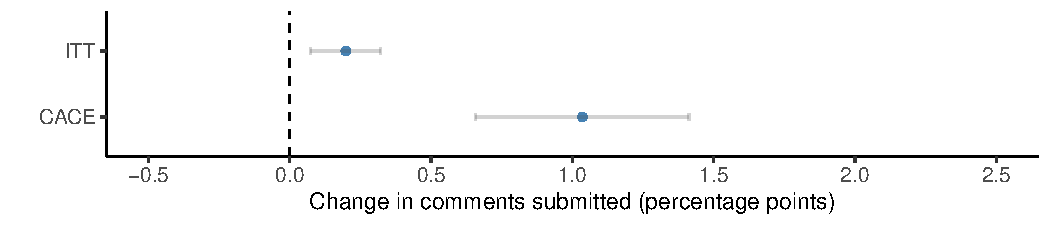
\includegraphics[width = \textwidth]{../figs/fgA6.pdf}
\caption{Intent-to-treat effect and complier average causal effect, all cities (without covariate adjustment)}
\label{fig: treatment_placebo_nocovs}
\end{figure}

\begin{figure}[H]
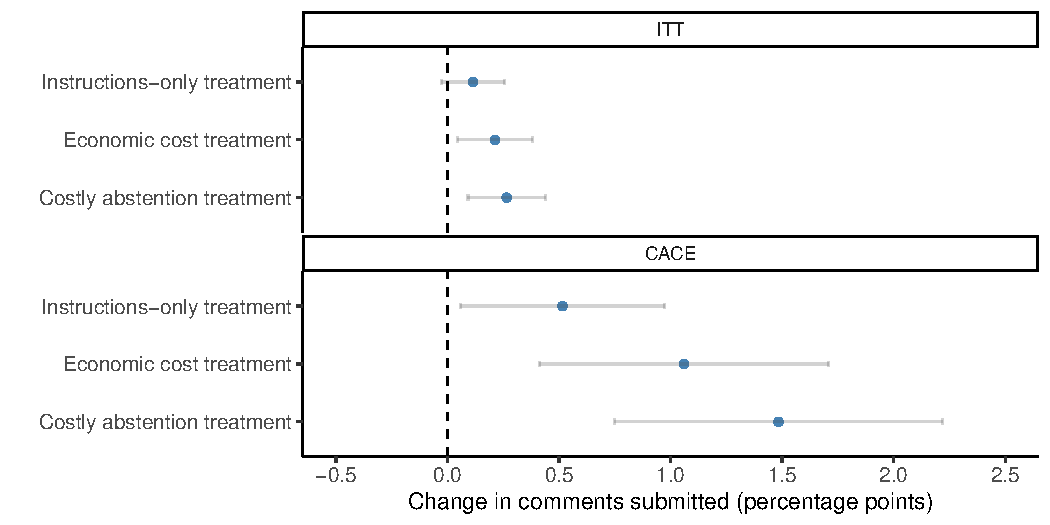
\includegraphics[width = \textwidth]{../figs/fgA7.pdf}
\caption{Effects by treatment group, all cities (without covariate adjustment)}
\label{fig: all_treatments_nocovs}
\end{figure}

\begin{table}[H]
\singlespace
\centering
\begin{tabular}{@{}llc@{}}
\toprule
\multicolumn{2}{c}{Estimand}          & p value \\ \midrule
CACE: & All treated vs. placebo       & 0.044   \\
CACE: & Instruction-only vs. placebo  & 0.386   \\
CACE: & Economic cost vs. placebo     & 0.071   \\
CACE: & Costly abstention vs. placebo & 0.011   \\
CACE: & Economic cost vs. instruction-only &   0.192 \\
CACE: & Costly abstention vs. instruction-only &  0.027 \\
CACE: & Costly abstention vs. economic cost & 0.315  \\
CACE: & Costly abstention  \& economic cost vs. instructions-only & 0.040 \\
ITT:  & All treated vs. placebo       & 0.091   \\
ITT:  & Instruction-only vs. placebo  & 0.403   \\
ITT:  & Economic cost vs. placebo     & 0.098   \\
ITT:  & Costly abstention vs. placebo & 0.033   \\ 
ITT: & Economic cost vs. instruction-only &   0.277 \\
ITT: & Costly abstention vs. instruction-only &  0.087 \\
ITT: & Costly abstention vs. economic cost & 0.532  \\
ITT: & Costly abstenion  \& economic cost vs. instructions-only & 0.112 \\
\bottomrule
\end{tabular}
\caption{Randomization inference p values}
\label{tab: ri}
\vspace{1mm}
{\setstretch{1}\textit{Note}: Randomization inference conducted using 10,000 simulations for CACEs and 1000 simulations for ITTs. Covariates not included due to computational demand.\par}
\end{table}




\begin{table}[H]
\centering
\resizebox{\linewidth}{!}{
\begin{tabular}[t]{lcccc}
\toprule
\multicolumn{1}{c}{ } & \multicolumn{2}{c}{All treatment groups vs. placebo} & \multicolumn{2}{c}{Individual treatments vs. placebo} \\
\cmidrule(l{3pt}r{3pt}){2-3} \cmidrule(l{3pt}r{3pt}){4-5}
  & ITT & CACE & ITT  & CACE \\
\midrule
\cellcolor[HTML]{D3D3D3}{Constant} & \cellcolor[HTML]{D3D3D3}{\num{-7.1987}***} & \cellcolor[HTML]{D3D3D3}{\num{-6.5439}***} & \cellcolor[HTML]{D3D3D3}{\num{-7.1987}***} & \cellcolor[HTML]{D3D3D3}{\num{-6.5439}***}\\
 & (\num{0.8168}) & (\num{1.4152}) & (\num{0.8168}) & (\num{1.4152})\\
 & {}[\num{-9.3648}, \num{-5.9318}] & {}[\num{-11.3781}, \num{-4.6301}] & {}[\num{-9.3648}, \num{-5.9318}] & {}[\num{-11.3781}, \num{-4.6301}]\\
\cellcolor[HTML]{D3D3D3}{Treated} & \cellcolor[HTML]{D3D3D3}{\num{1.2239}+} & \cellcolor[HTML]{D3D3D3}{\num{1.9864}*} & \cellcolor[HTML]{D3D3D3}{} & \cellcolor[HTML]{D3D3D3}{}\\
 & (\num{0.8302}) & (\num{1.4265}) &  & \\
 & {}[\num{-0.0850}, \num{3.4045}] & {}[\num{0.0265}, \num{6.8285}] &  & \\
\cellcolor[HTML]{D3D3D3}{Instructions-only treatment} & \cellcolor[HTML]{D3D3D3}{} & \cellcolor[HTML]{D3D3D3}{} & \cellcolor[HTML]{D3D3D3}{\num{0.8548}} & \cellcolor[HTML]{D3D3D3}{\num{1.3414}}\\
 &  &  & (\num{0.8733}) & (\num{1.4784})\\
 &  &  & {}[\num{-0.5931}, \num{3.0816}] & {}[\num{-0.8391}, \num{6.2197}]\\
\cellcolor[HTML]{D3D3D3}{Economic cost treatment} & \cellcolor[HTML]{D3D3D3}{} & \cellcolor[HTML]{D3D3D3}{} & \cellcolor[HTML]{D3D3D3}{\num{1.3048}+} & \cellcolor[HTML]{D3D3D3}{\num{2.0372}+}\\
 &  &  & (\num{0.8532}) & (\num{1.4489})\\
 &  &  & {}[\num{-0.0776}, \num{3.5102}] & {}[\num{-0.0157}, \num{6.8950}]\\
\cellcolor[HTML]{D3D3D3}{Costly abstention treatment} & \cellcolor[HTML]{D3D3D3}{} & \cellcolor[HTML]{D3D3D3}{} & \cellcolor[HTML]{D3D3D3}{\num{1.4797}*} & \cellcolor[HTML]{D3D3D3}{\num{2.3874}*}\\
 &  &  & (\num{0.8477}) & (\num{1.4368})\\
 &  &  & {}[\num{0.1150}, \num{3.6792}] & {}[\num{0.3850}, \num{7.2367}]\\
\midrule
Num.Obs. & \num{19951} & \num{3381} & \num{19951} & \num{3381}\\
\bottomrule
\multicolumn{5}{l}{\rule{0pt}{1em}+ p $<$ 0.1, * p $<$ 0.05, ** p $<$ 0.01, *** p $<$ 0.001}\\
\multicolumn{5}{l}{\rule{0pt}{1em}Notes: Standard errors clustered at the address level in parentheses. 95 percent confidence intervals in brackets.}\\
\end{tabular}}
\end{table}

\captionof{table}{ITT and CACE estimates from penalized maximum likelihood}
\label{tab: pml}

\begin{figure}[!htb]
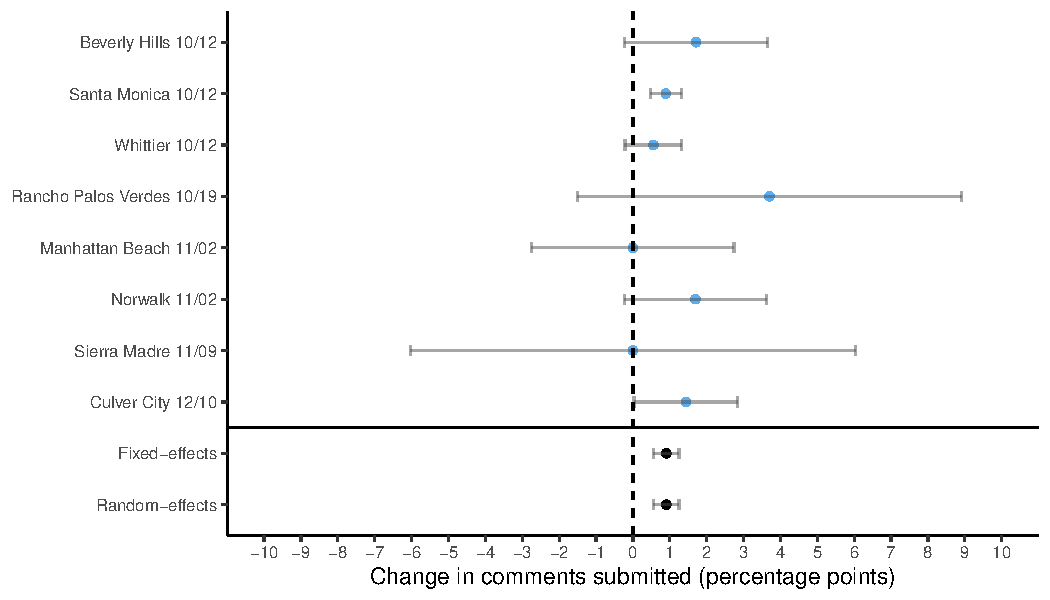
\includegraphics[width = \textwidth]{../figs/fgA8.pdf}
\caption{Meta-analysis of complier average causal effects by city, excluding pilot studies}
\label{fig: meta_nopilot}
\end{figure}

\begin{figure}[!htb]
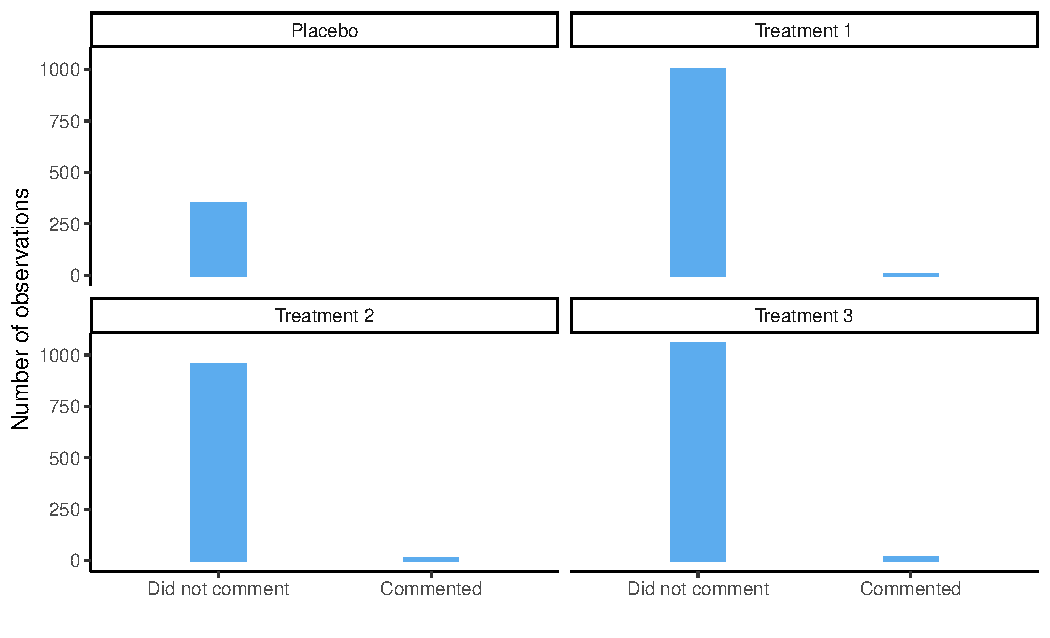
\includegraphics[width = \textwidth]{../figs/fgA9.pdf}
\caption{Distribution of outcomes by treatment group (compliers only)}
\label{fig: outcomes}
\end{figure}

\clearpage

The Bayes factors in \hyperref[sec: results_group]{the results section} are computed for hypotheses that the differences between treatments are greater than zero (e.g., costly abstention treatment - instructions only treatment $>$ 0) and its alternative using the Savage-Dickey density ratio method. The Bayes factors are 97 and 5 for the costly abstention treatment vs. the instructions only treatment and costly abstention treatment vs. economic cost treatment, respectively. The posterior probability exceeds 95\% for a one-sided hypothesis test in both comparisons, and exceeds 95\% for a two-sided test in the first comparison. Given that the directionality and relative magnitudes of the treatment effects were pre-registered and negative treatment effects are theoretically implausible, a one-sided hypothesis test seems reasonable. 

\begin{figure}[!htb]
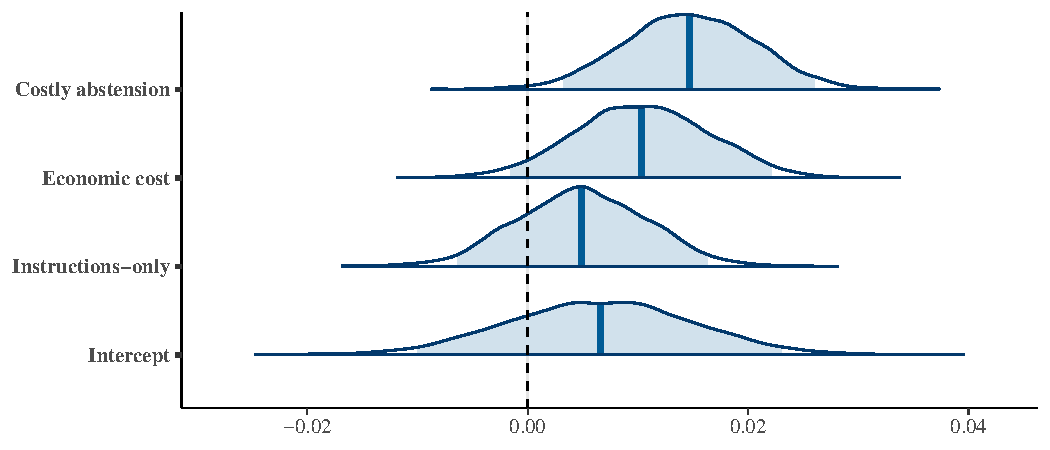
\includegraphics[width = \textwidth]{../figs/fgA10.pdf}
\caption{Bayesian multilevel model: coefficient estimates and posterior distributions (includes city fixed effects)}
\label{fig: bayes_coef}
\end{figure}

\begin{figure}[!htb]
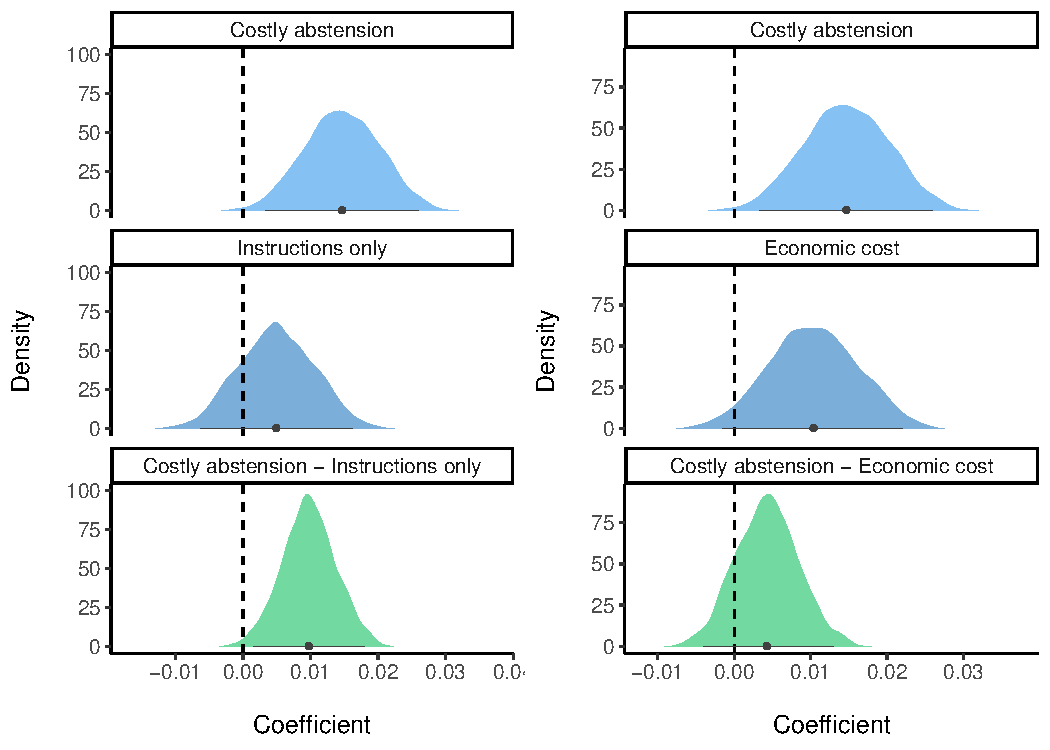
\includegraphics[width = \textwidth]{../figs/fgA11.pdf}
\caption{Posterior distributions of costly abstention treatment, instructions only treatment, and difference}
\label{fig: posterior_dists}
\end{figure}

\end{document} 